\documentclass[xcolor=table, 11pt, aspectratio=1610]{beamer}

%\usepackage{arev}
\usepackage{amsmath,amssymb,amscd}
\usepackage{dsfont}
\usepackage{mathrsfs}
\usepackage{yfonts}
\usepackage{bm}
\usepackage{graphicx}
\usepackage{tabularx}
\usepackage{animate}
\usepackage{listings}
\usepackage{pifont}
\usepackage{ulem}
% \usepackage{mathtools}
%\usepackage{ifthen}

%\usepackage{xeCJK}
%\usepackage{fontspec}
%\newfontfamily\cjkfont{PingFang SC}
%\setCJKmainfont{PingFang SC}
\newcolumntype{x}{>{\centering\arraybackslash}X}
\renewcommand{\arraystretch}{1.5}
\newcommand{\uone}{\mathrm U(1)}
\DeclareMathOperator{\img}{img}
\DeclareMathOperator{\hhom}{Hom}

\usepackage{tikz}
	\usetikzlibrary{calc}
	\usetikzlibrary{arrows,shapes, positioning, matrix}
	\usetikzlibrary{decorations.markings}
	\tikzset{>=stealth}
	\tikzstyle arrowstyle=[scale=1]
	\tikzstyle directed=[postaction={decorate,decoration={markings,
 	   mark=at position .15 with {\arrow[arrowstyle]{stealth}}}}]
\tikzstyle string=[thick,postaction={decorate,decoration={markings,
    mark=at position .55 with {\arrow[arrowstyle]{stealth}}}}]
\tikzstyle dual_string=[dashed,postaction={decorate,decoration={markings,
    mark=at position .55 with {\arrow[arrowstyle]{stealth}}}}]

\tikzstyle dw=[thick,postaction={decorate,decoration={markings,
    mark=at position 1 with {\arrow[arrowstyle]{stealth}}}}]
\tikzstyle group=[mbg]
\newcommand*{\halfway}{0.5*\pgfdecoratedpathlength+.5*8pt}\tikzstyle arrowstyle=[scale=1]
\newcommand*{\halfwayb}{0.5*\pgfdecoratedpathlength}
\tikzstyle arrowstyle=[scale=1]
\tikzstyle fermion=[thick,postaction={decorate},decoration={markings,
    mark=at position \halfway with {\arrow[arrowstyle]{latex}}}]
\tikzstyle fermion2=[thick,postaction={decorate},decoration={markings,
        mark=at position \halfwayb with {\arrow[arrowstyle]{latex}}}]

\usepackage{pgffor}
\newcommand{\mb}[1]{\mathbf{#1}}
\renewcommand{\cal}[1]{\mathcal{#1}}

\newcommand{\ag}[2]{#1_\mb{#2}}
\newcommand{\cohosub}[1]{\scalebox{0.72}{\textswab{#1}}}
\newcommand{\cohosubsub}[1]{\scalebox{0.6}{\textswab{#1}}}
\newcommand{\coho}[1]{\textswab{#1}}

\DeclareMathOperator{\tr}{Tr}
\DeclareMathOperator{\im}{Im}
\DeclareMathOperator{\re}{Re}

\mode<presentation>
{
  %\usetheme{Warsaw}
  % or ...
  %\useoutertheme{rectangle}
  \setbeamertemplate{frametitle}[default][center]
  \defbeamertemplate{itemize item}{flat}{\begin{pgfpicture}{-1ex}{0ex}{1ex}{2ex}
      \pgfpathcircle{\pgfpoint{0pt}{.6ex}}{0.6ex}
      \pgfusepath{fill}
    \end{pgfpicture}%
  }
  \defbeamertemplate{itemize subitem}{flat}{\footnotesize\raise0.5pt\hbox{\textbullet}}
  \defbeamertemplate{itemize subsubitem}{flat}{\footnotesize\raise0.5pt\hbox{\textbullet}}

  %\useinnertheme{circles}
  \setbeamertemplate{items}[flat]
  \setbeamertemplate{sections/subsections in toc}[circle]
  \setbeamertemplate{blocks}[rounded]
  \setbeamertemplate{title page}[default][colsep=-4bp,rounded=true]
  \setbeamertemplate{part page}[default][colsep=-4bp,rounded=true]
  \setbeamercovered{transparent}
  %\usecolortheme{spruce}
  %\definecolor{THU}{RGB}{116,61,130}
  \definecolor{mbg}{RGB}{0,0,160}
  \setbeamercolor*{palette primary}{fg=white,bg=mbg}
  \setbeamercolor*{titlelike}{parent=palette primary}
  \setbeamercolor*{structure}{fg=mbg}
  \setbeamercolor{frametitle}{fg=white,bg=mbg}
  % or whatever (possibly just delete it)
  \setbeamercolor{block title}{bg=mbg,fg=white}
  \setbeamercolor{block body}{bg=mbg!15}


  \addtobeamertemplate{navigation symbols}{}{ \hspace{1em}%
    \usebeamerfont{footline}%
    \insertframenumber / \inserttotalframenumber }
}


%\usepackage[english]{babel}
% or whatever

%\usepackage[latin1]{inputenc}
% or whatever

%\usepackage{times}
%\usepackage[T1]{fontenc}
% Or whatever. Note that the encoding and the font should match. If T1
% does not look nice, try deleting the line with the fontenc.

\title[Space-group SPTs] % (optional, use only with long paper titles)
{Towards a classification of fermionic crystalline SPT states}

\author[Y Qi] % (optional, use only with lots of authors)
{Yang~Qi}
% - Give the names in the same order as the appear in the paper.
% - Use the \inst{?} command only if the authors have different
%   affiliation.

\institute[Fudan] % (optional, but mostly needed)
{Department of Physics, Fudan University, Shanghai, China.}
% - Use the \inst command only if there are several affiliations.
% - Keep it simple, no one is interested in your street address.

%\date{2016 Annual Meeting of Fudan CFTPP} % (optional, should be abbreviation of conference name)
%{Fudan University, Oct 13 2015}
%\date{Hong Kong Forum of Physics, HKU, Jan 7-9, 2019.}
%\date{QuIST V, Kunming, Aug. 2nd, 2019.}
%\date{Perimeter Institute, Sept. 3rd, 2019.}
%\date{Beihang University, Oct. 22nd, 2019.}
\date{Simons Center for Geometry and Physics, May 2021.}
% - Either use conference name or its abbreviation.
% - Not really informative to the audience, more for people (including
%   yourself) who are reading the slides online

\subject{Theoretical Physics}
% This is only inserted into the PDF information catalog. Can be left
% out.



% If you have a file called "university-logo-filename.xxx", where xxx
% is a graphic format that can be processed by latex or pdflatex,
% resp., then you can add a logo as follows:

\pgfdeclareimage[height=1cm]{university-logo}{../resources/fudan}
\logo{\pgfuseimage{university-logo}}

\AtBeginSection[]
{
\begin{frame}{Outline}
%	\begin{columns}
%		\begin{column}[t]{.45\textwidth}
%		\begin{center}
%			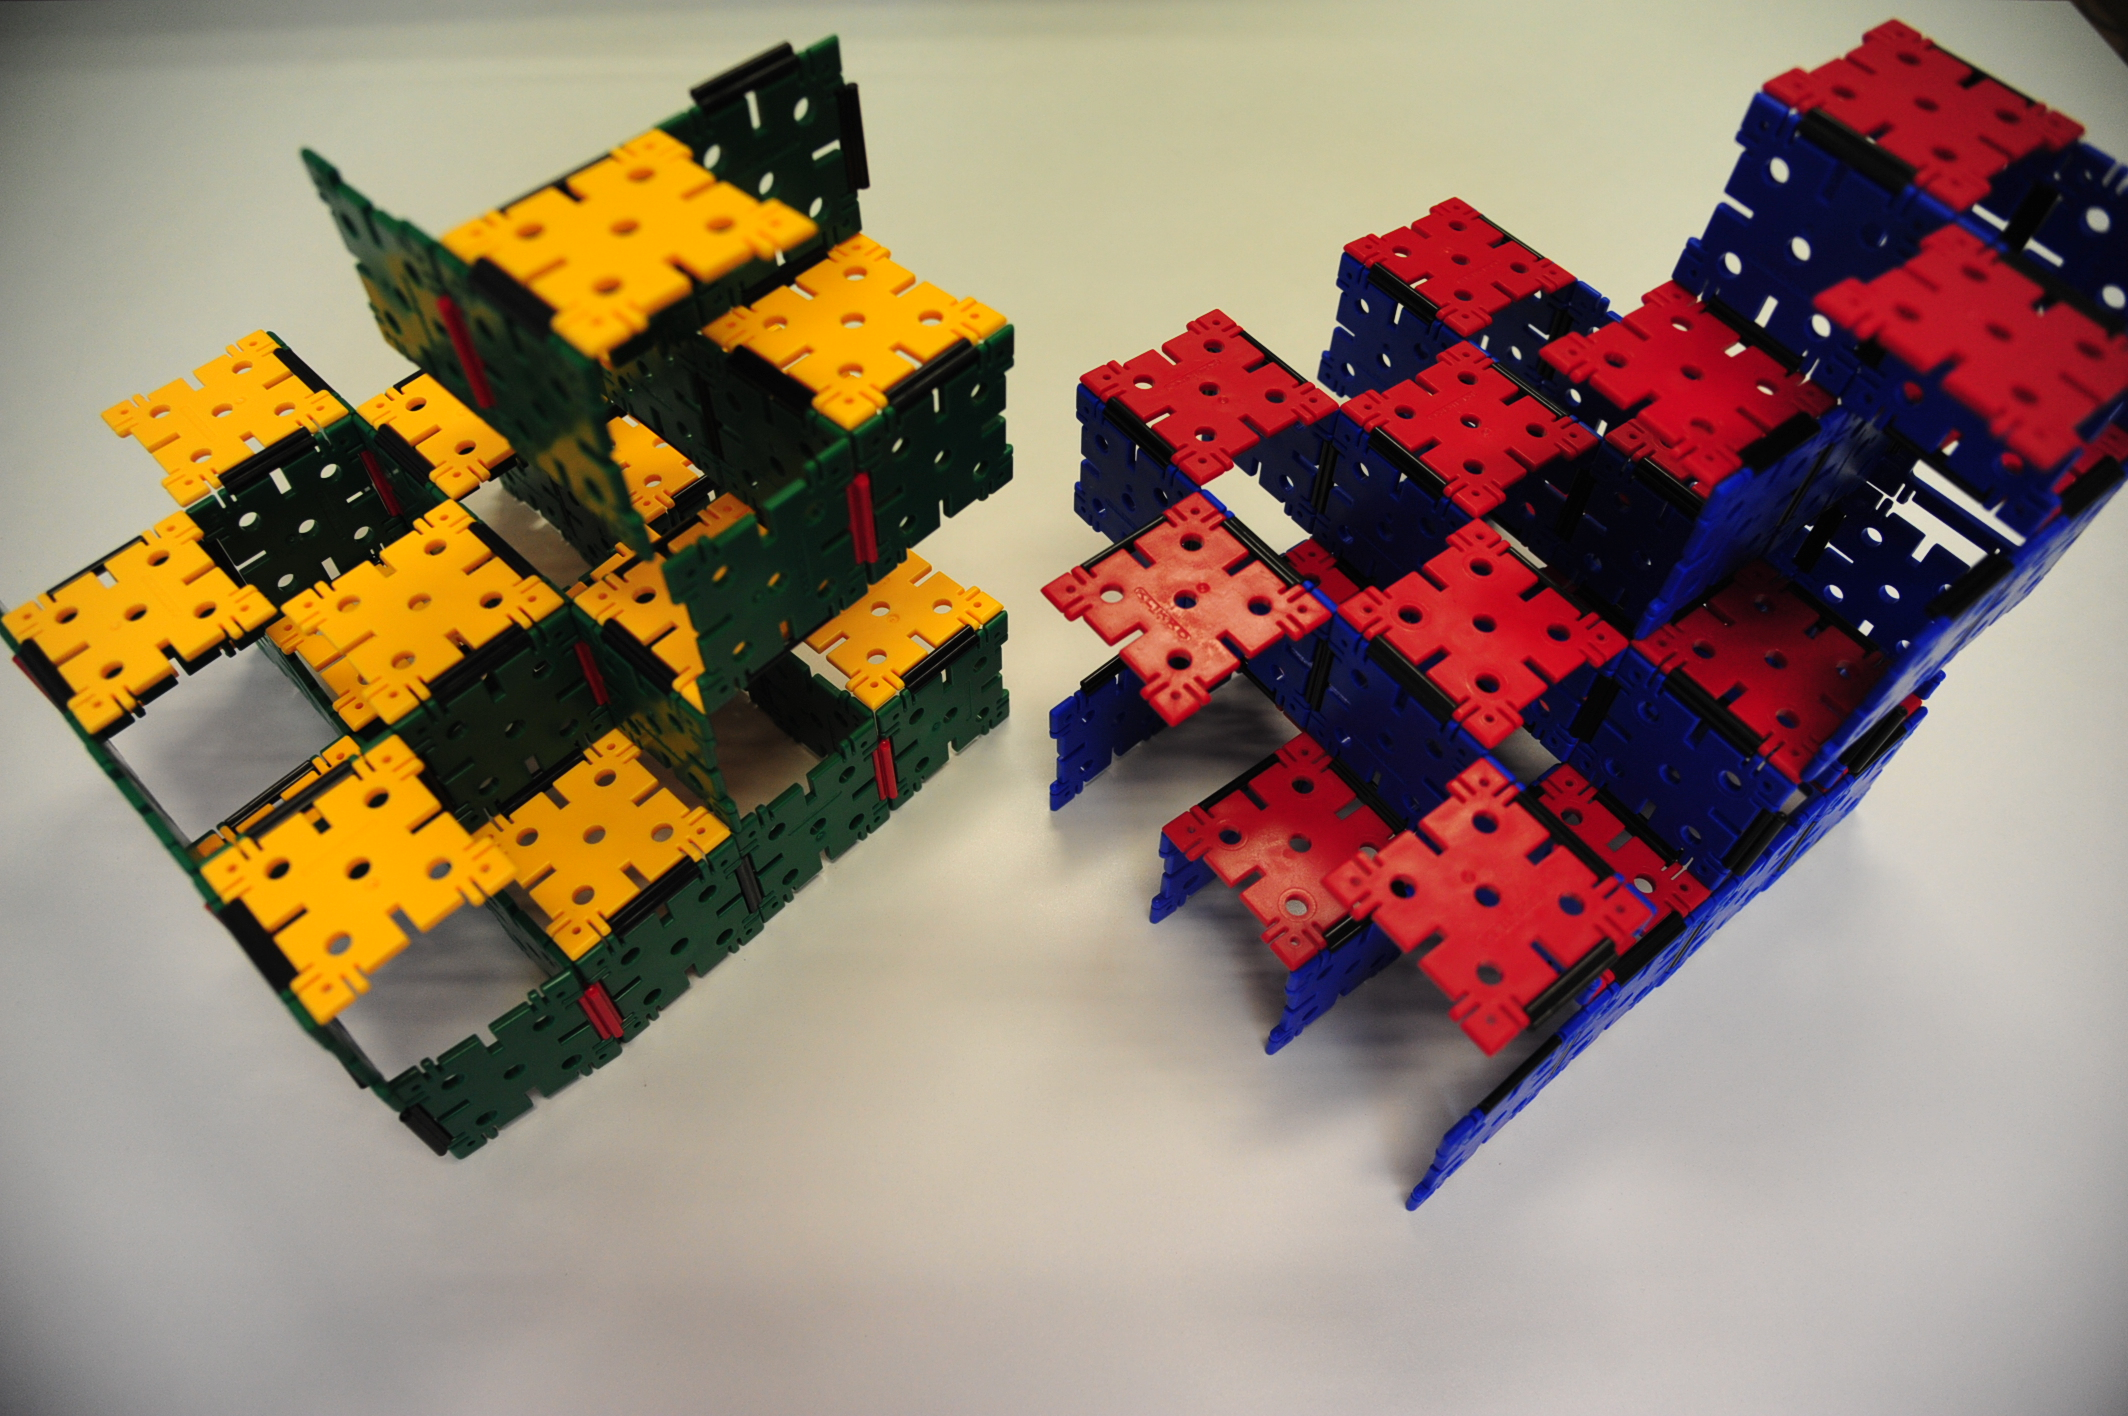
\includegraphics[height=4cm]{toys}
%		\end{center}
%	\end{column}
%	\begin{minipage}[t][0.5\textheight]{0.55\textwidth}
      \tableofcontents[currentsection]
%    \end{minipage}\hfill
%	\end{columns}
\end{frame}
}


% Delete this, if you do not want the table of contents to pop up at
% the beginning of each subsection:

\begin{document}

\begin{frame}
  \titlepage
\end{frame}

\begin{frame}{Collaborators}
  \begin{itemize}
  \item Yunqing Ouyang: Fudan University.
  \item Zhi-Da Song: Princeton University $\Rightarrow$ Beijing University.
  \item Qing-Rui Wang: Tsinghua University.
  \item Chen Fang: Institute of Physics, Beijing.
  \item Zheng-Cheng Gu: Chinese University of Hong Kong.
    \begin{center}
      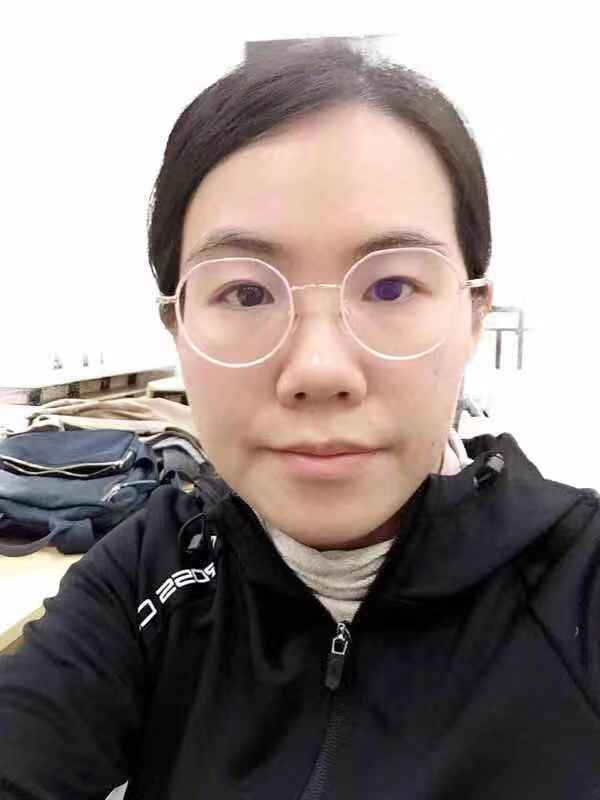
\includegraphics[height=2.5cm]{../people/yunqing}
      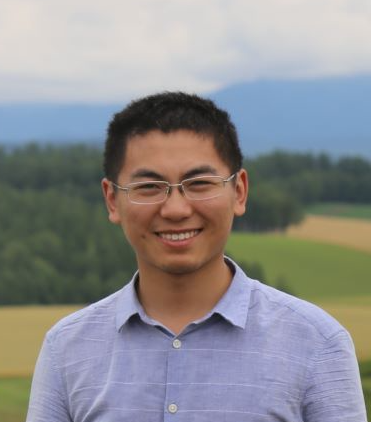
\includegraphics[height=2.5cm]{../people/zhidasong}
      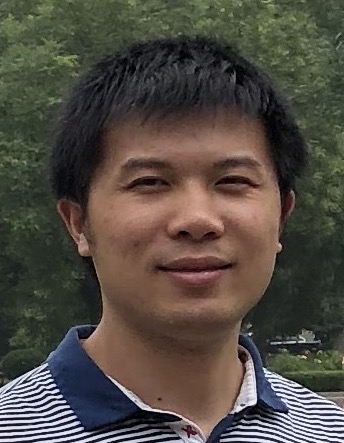
\includegraphics[height=2.5cm]{../people/qingrui}      
      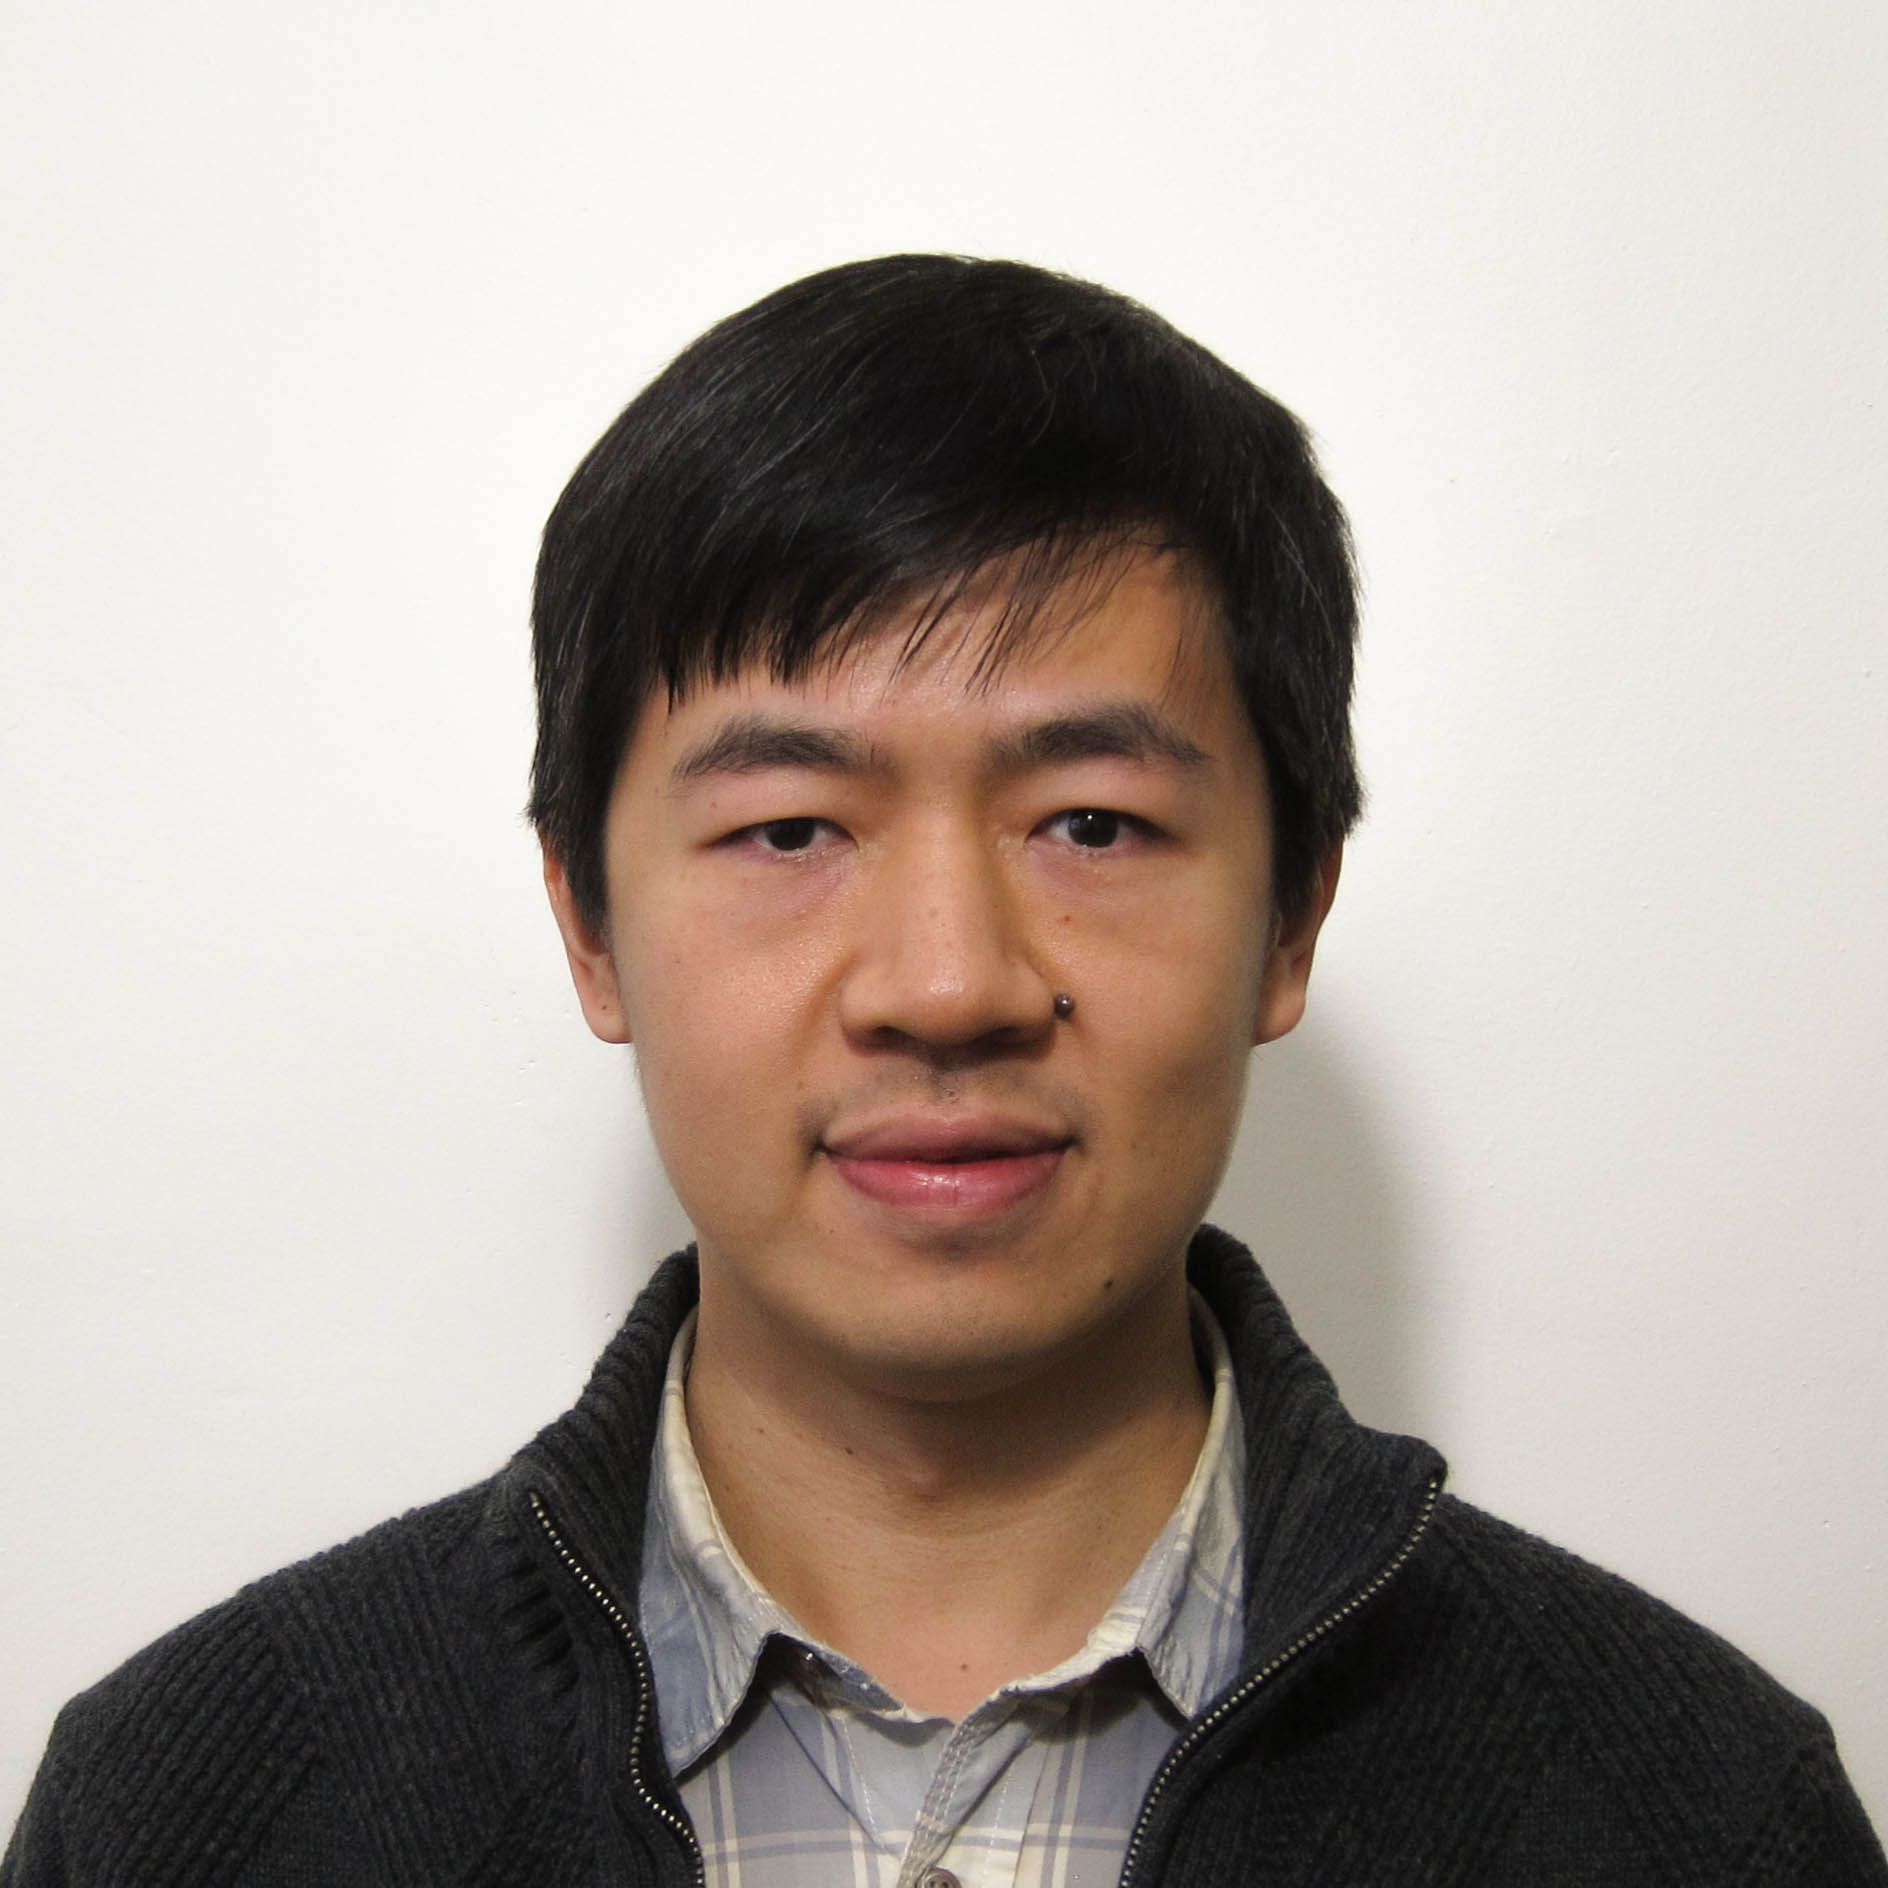
\includegraphics[height=2.5cm]{../people/chenfang}
      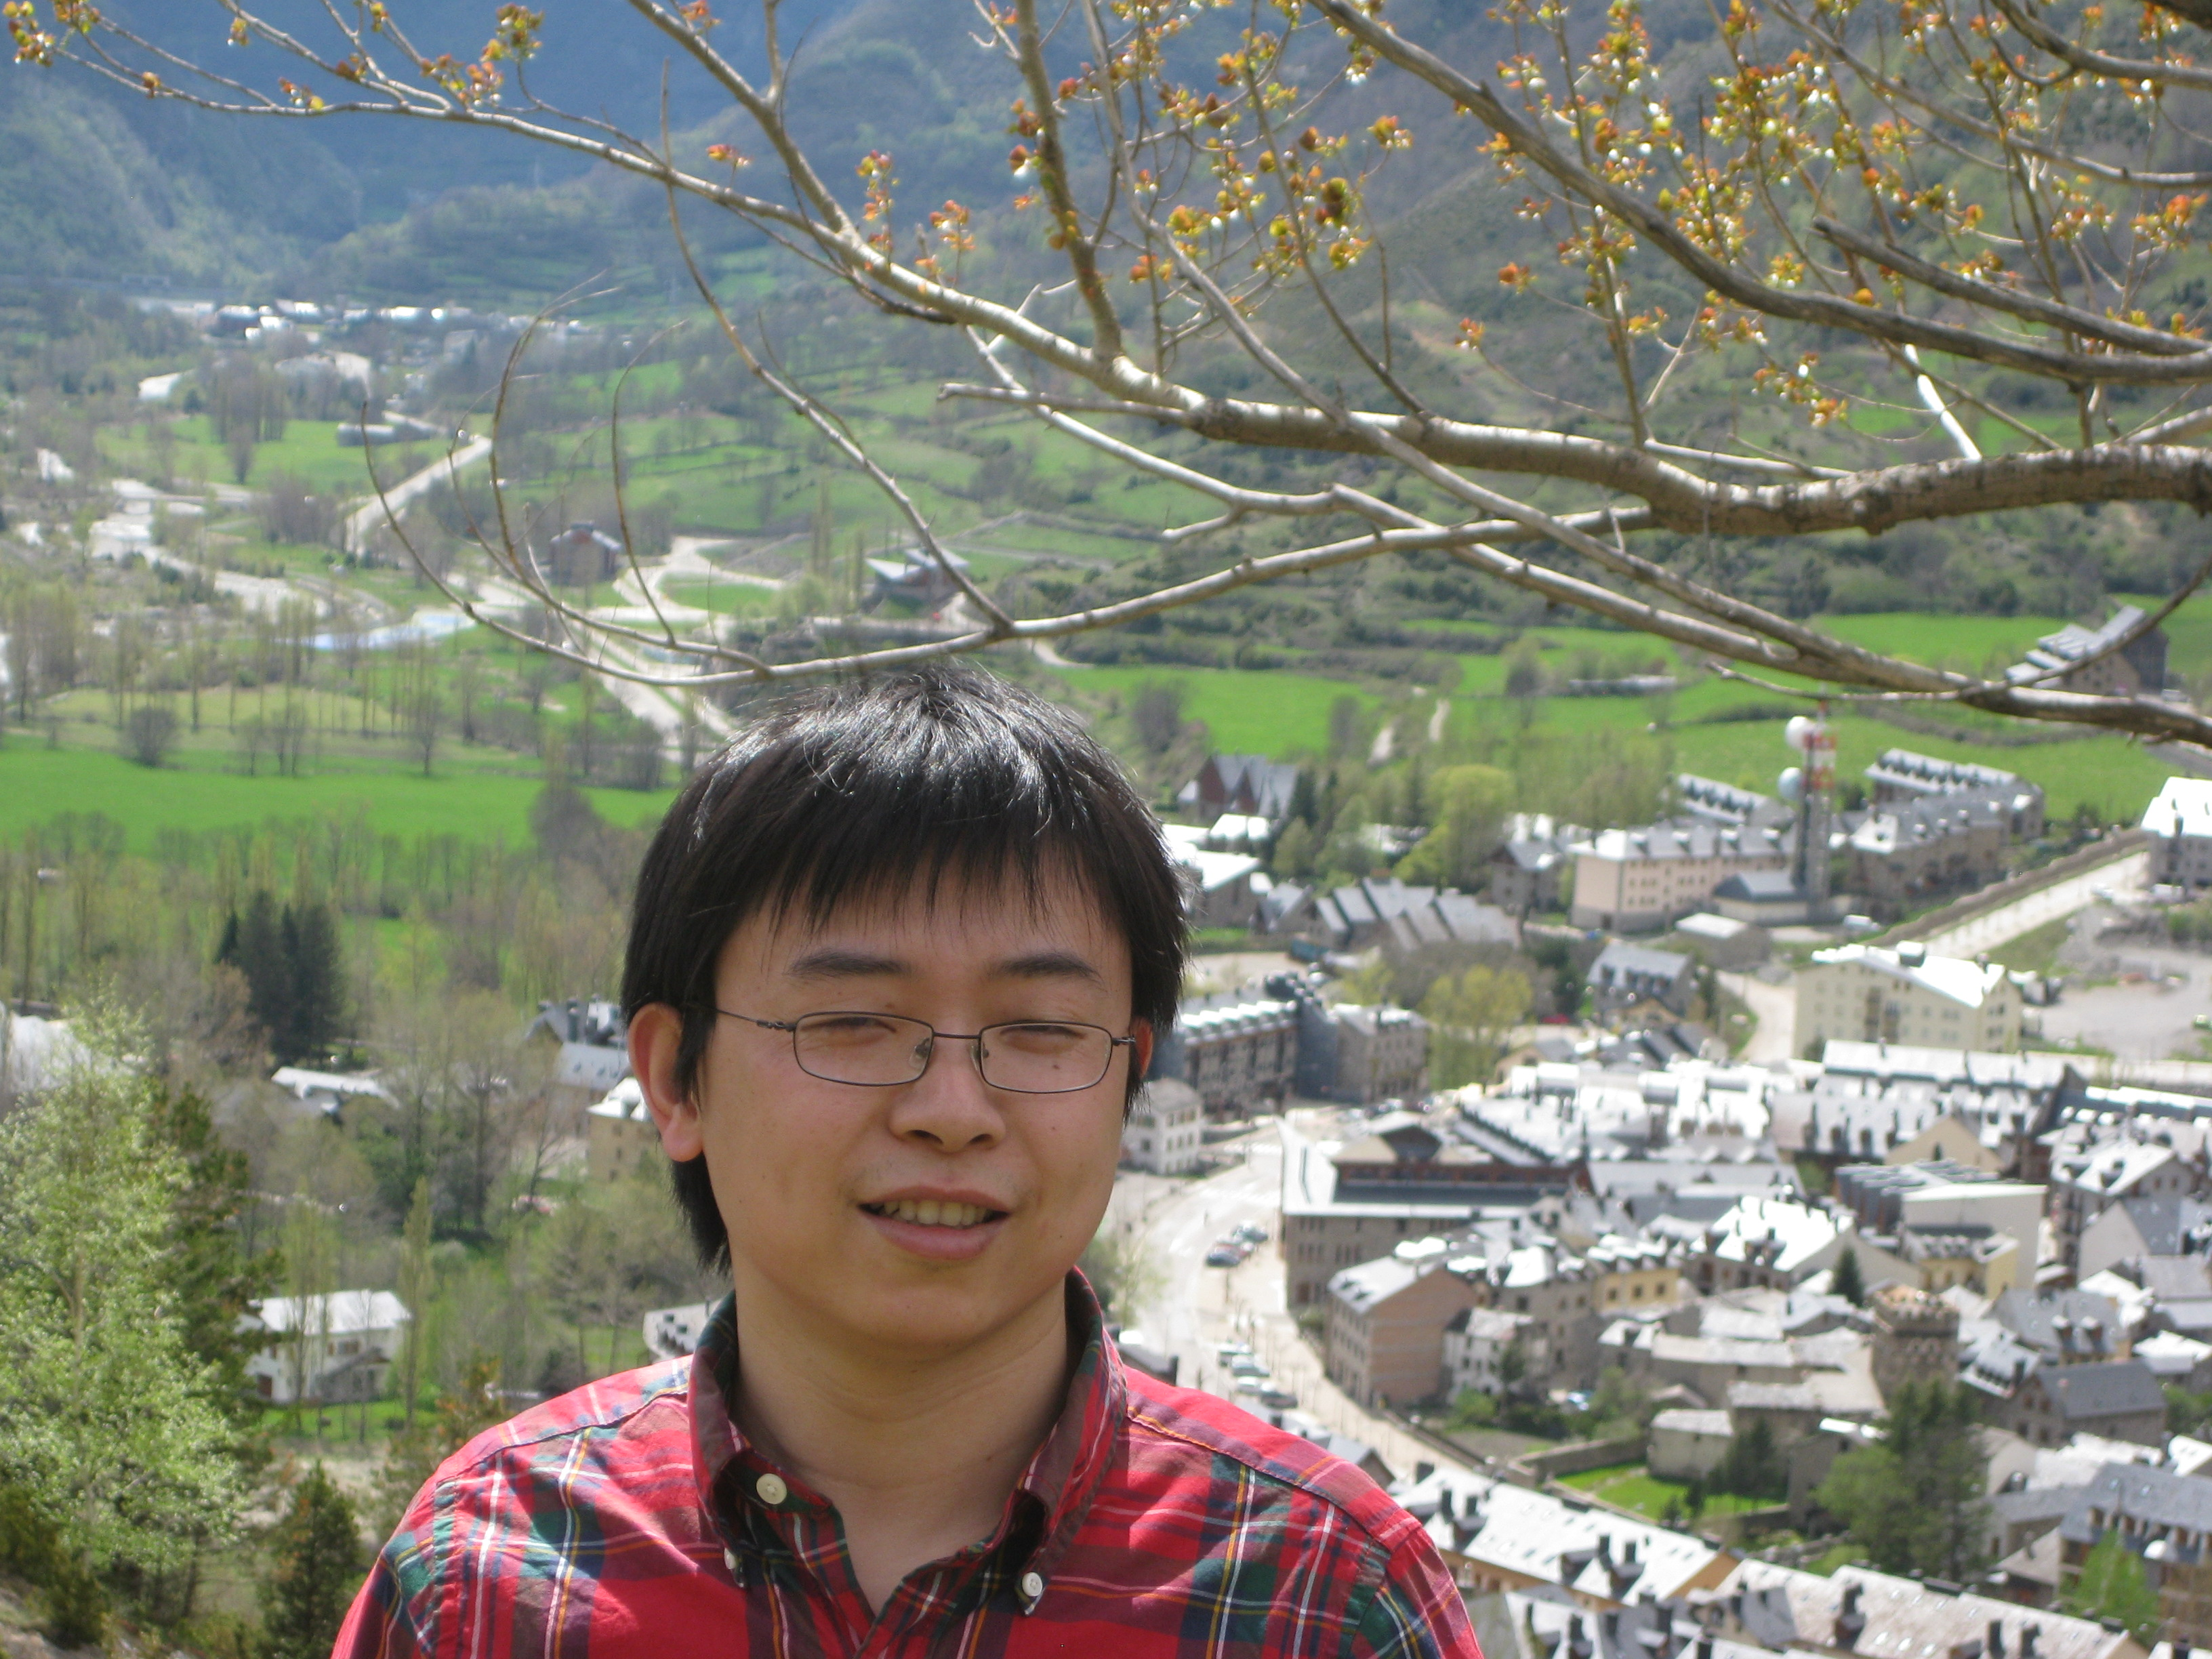
\includegraphics[height=2.5cm]{../people/zhengcheng}
    \end{center}
  \item Zhida Song, Chen Fang and YQ, Nature Communications \textbf{11} 4197 (2020).
  \item Yunqing Ouyang, Qing-Rui Wang, Zheng-Cheng Gu and YQ, arXiv:2005.06572.
\end{itemize}
\end{frame}

\begin{frame}{Outline}
%	\begin{columns}
%		\begin{column}[t]{.45\textwidth}
%		\begin{center}
%			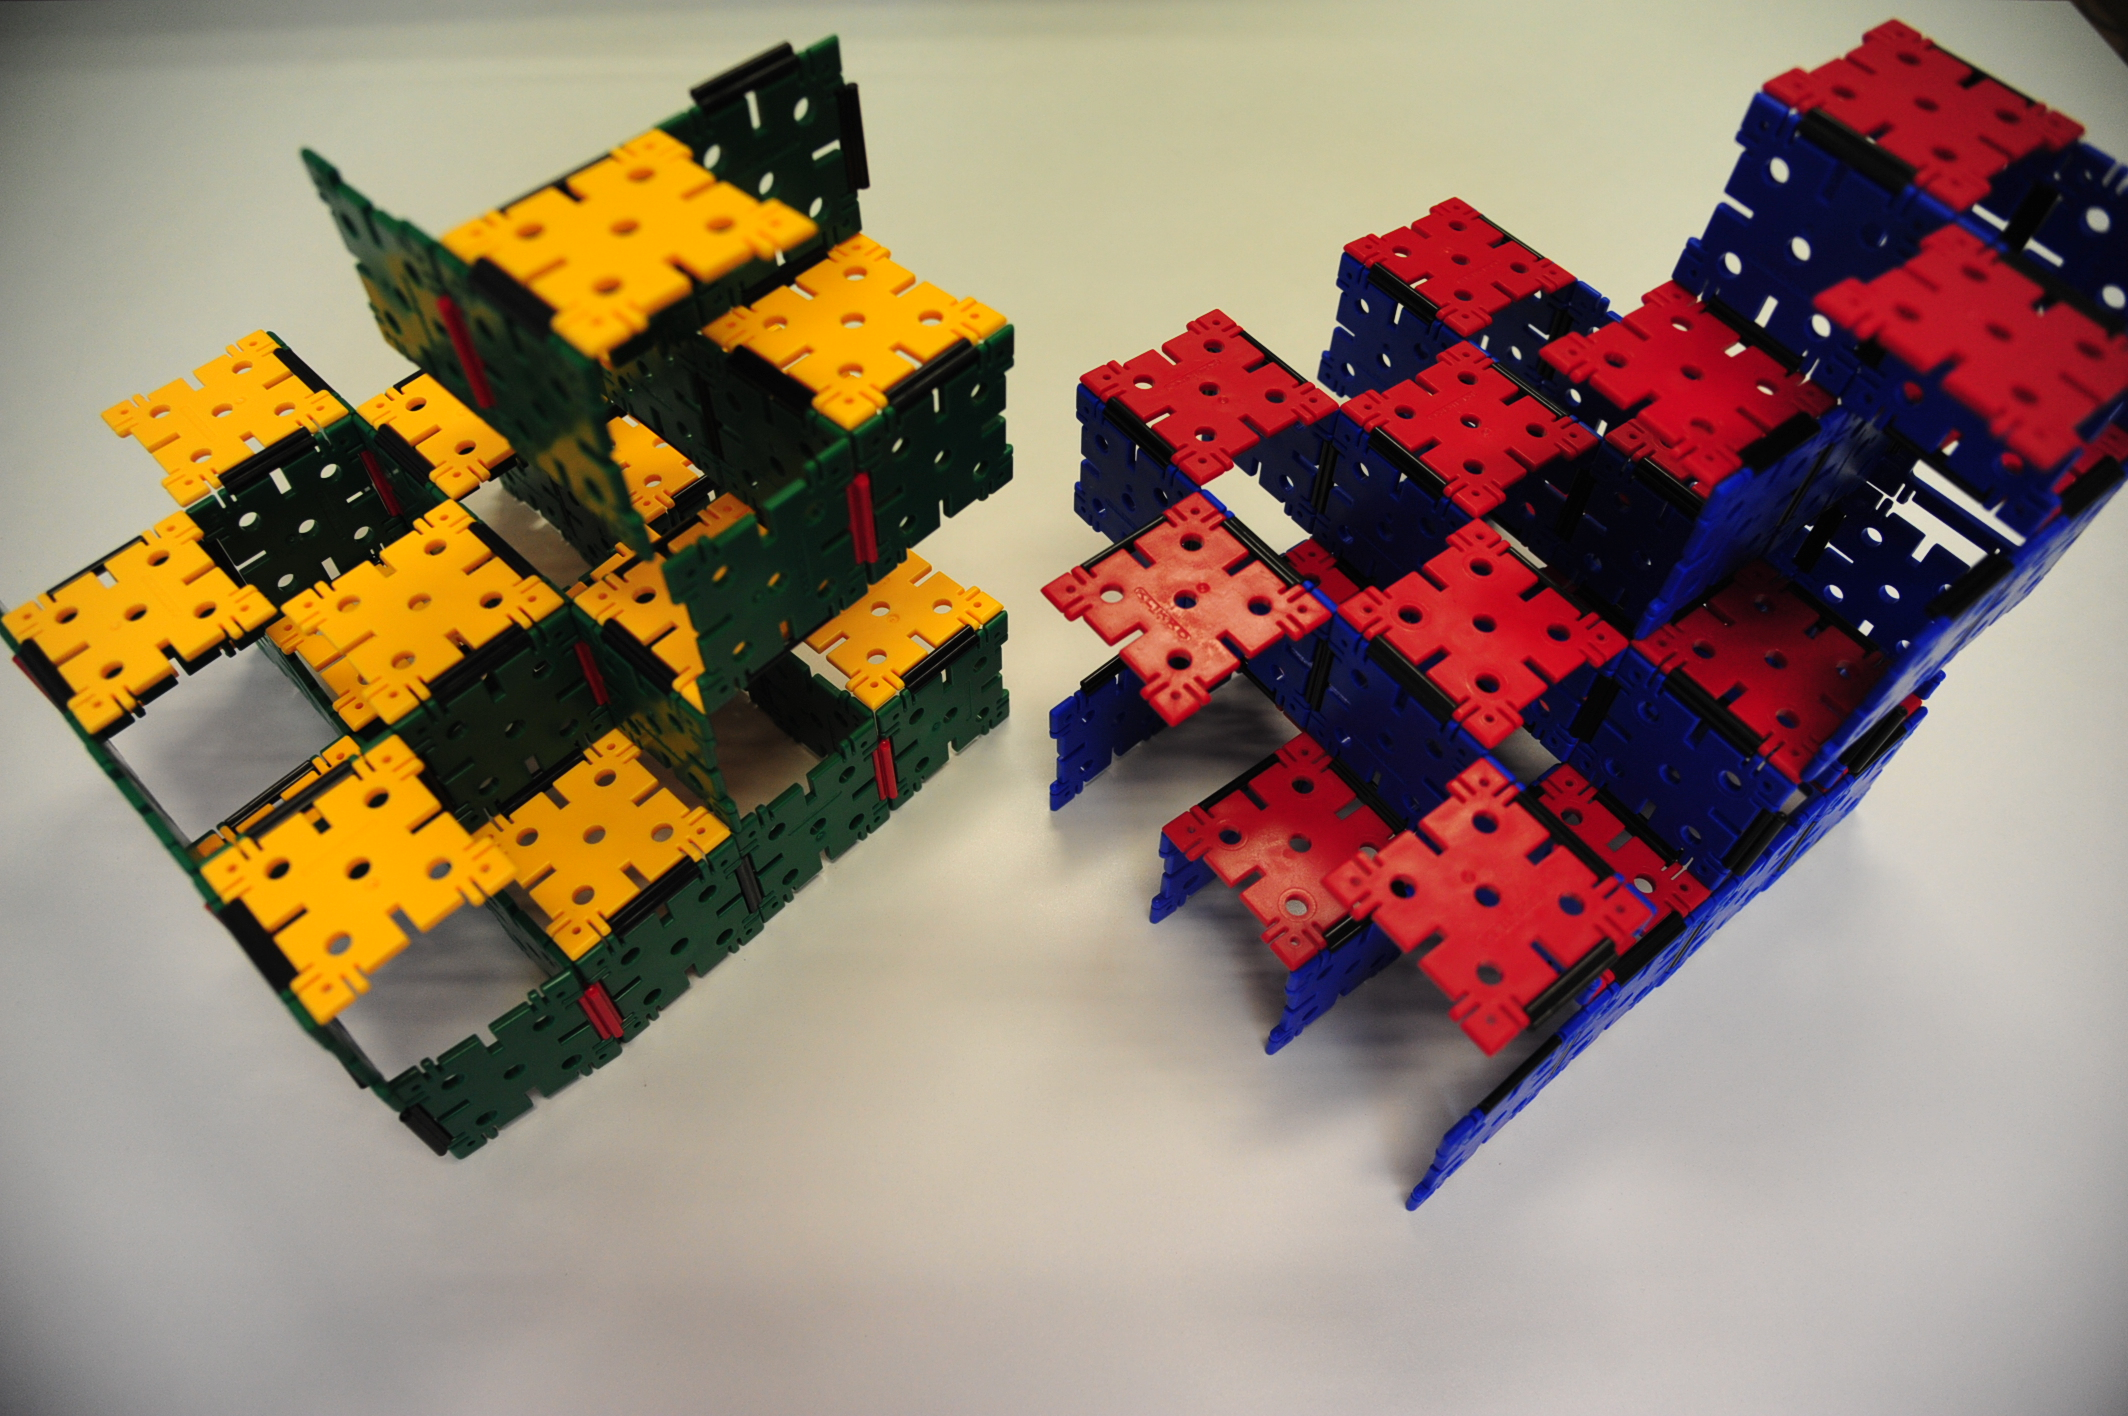
\includegraphics[height=4cm]{toys}
%		\end{center}
%	\end{column}
%	\begin{minipage}[t][0.5\textheight]{0.55\textwidth}
      \tableofcontents
%    \end{minipage}\hfill
%	\end{columns}
\end{frame}


\section{Introduction to SPT States}

\begin{frame}
  \frametitle{Symmetry-Protected Topological (SPT) states}
\begin{itemize}
\item SPT: gapped topological phases beyond Landau paradiam.
\item Gapped bulk : cannot be smoothly connected to a trivial state without closing gap or breaking symmetry.
\item Symmetry-protected gapless surface states.
\item Free-fermion states: topological insulators, topological superconductors: $K$-theory.
\item Bosonic SPTs: Haldane chain, CZX/Levin-Gu state, etc: Group Cohomology.
\item Interacting fermionic SPTs.
\end{itemize}
\end{frame}

%\begin{frame}
%  \frametitle{Abelian-group classification}
%  \begin{itemize}
%  \item SPT phases and boundary anomalies are classified by Abelian groups ($\mathbb Z$ or $\mathbb Z_n$).
%    \begin{itemize}
%    \item Addition: stacking of phases/gapless boundaries.
%    \item 0: The trivial phase/gapped boundary.
%    \end{itemize}
%  \item 2D Chern-insulators (Integer Quantum Hall):
%    \begin{center}
%      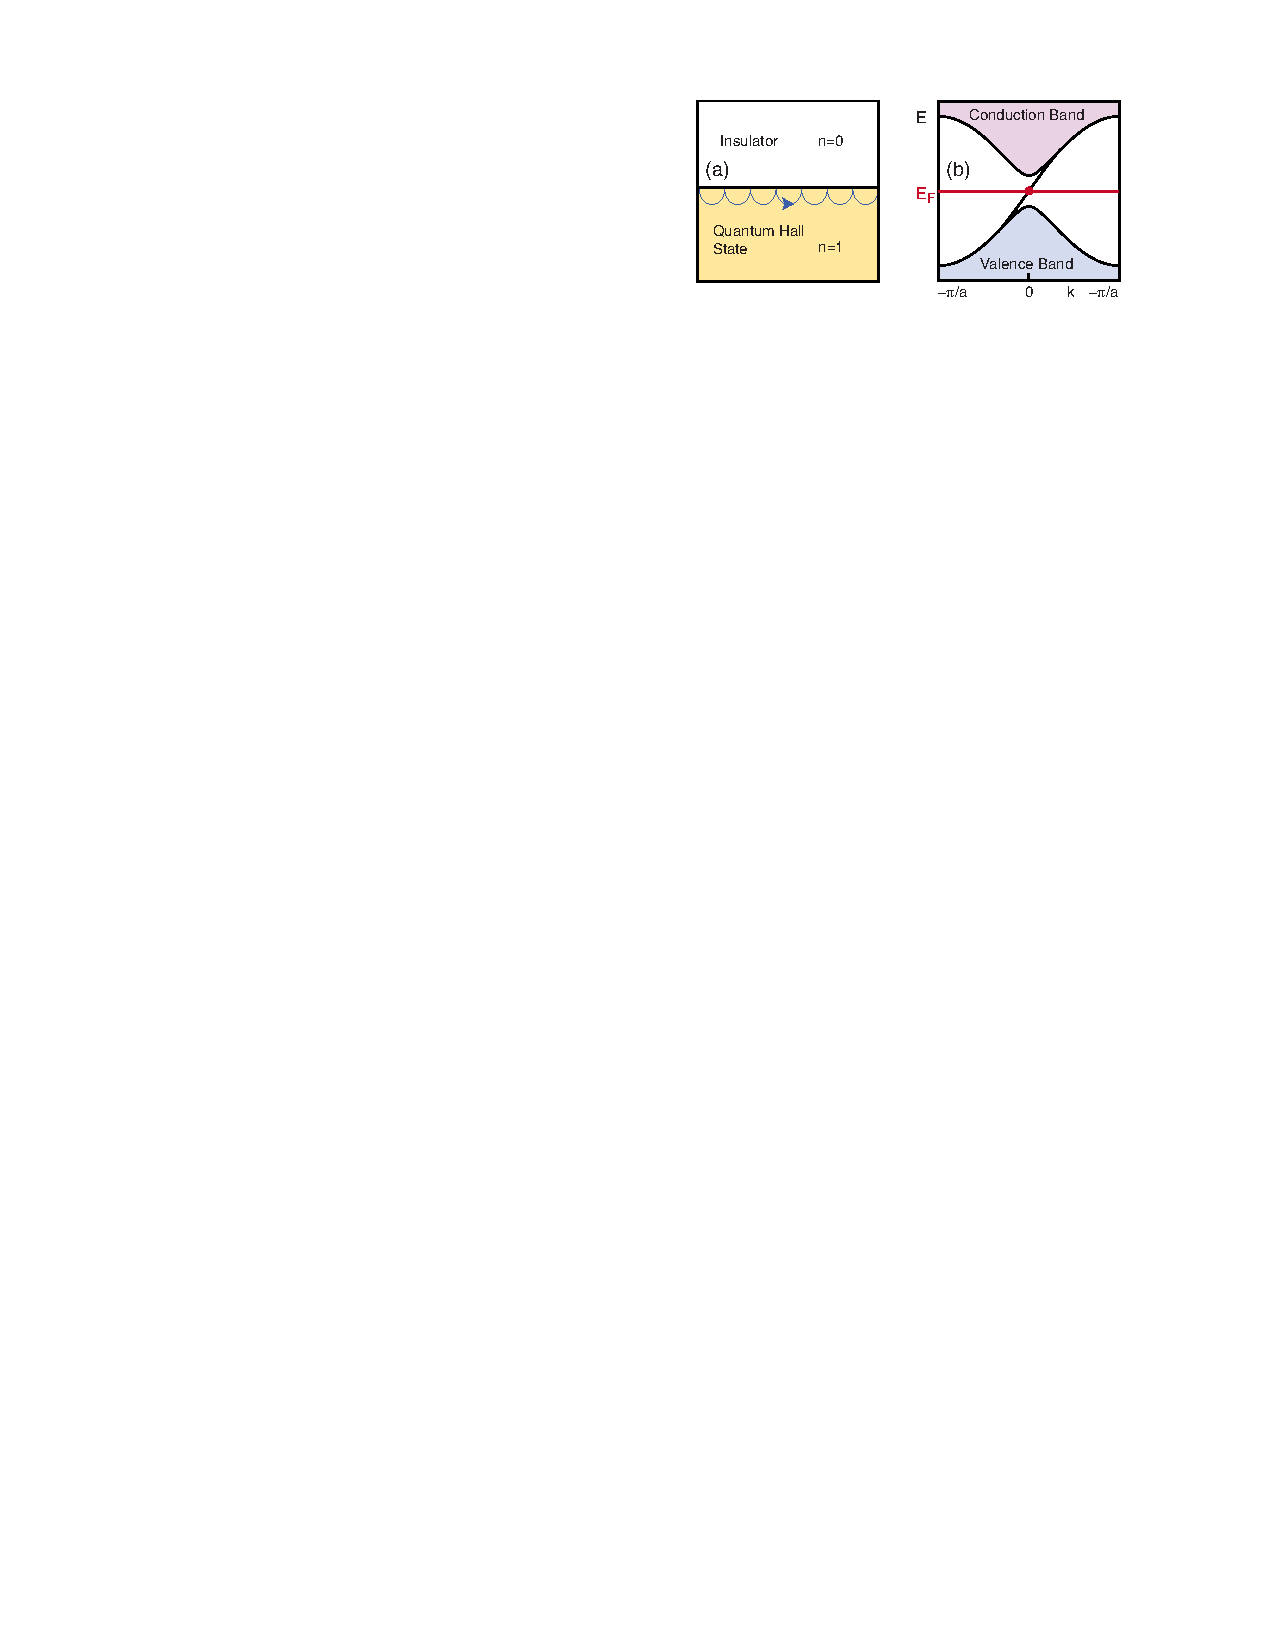
\includegraphics[width=8cm]{qhe_edge}
%    \end{center}
%    Classified by $\mathbb Z$: $[n]+[m]=[n+m]$; $[n]+[-n] = 0$.
%  \end{itemize}
%\end{frame}

%\begin{frame}
%	\frametitle{Abelian-group classification}
%	\begin{itemize}
%		\item 3D Topological Insulators:
%		\begin{center}
%			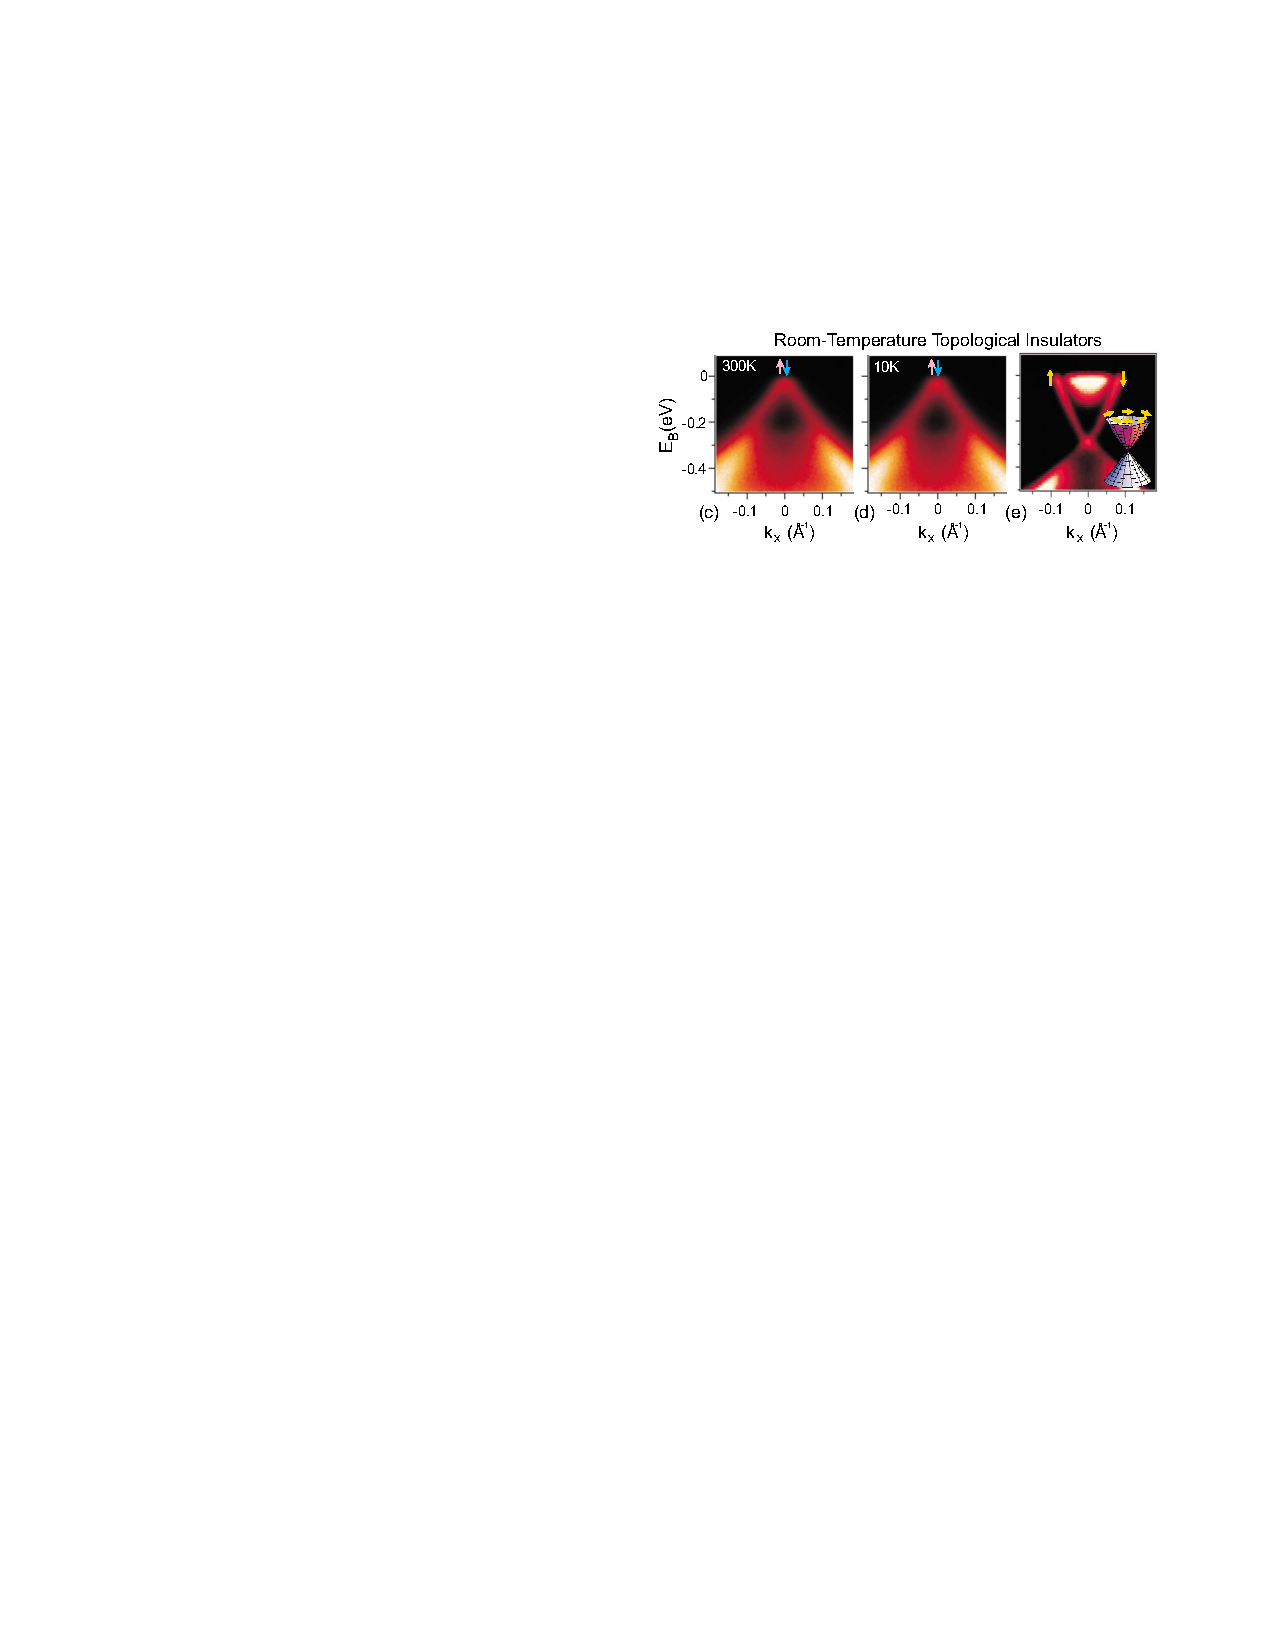
\includegraphics[width=8cm]{ti_surface}
%		\end{center}
%		Classified by $\mathbb Z_2$: $[1]+[1] = 0$.
%		\item 1D Haldane chain:
%		\begin{center}
%			
\includegraphics[width=6cm]{../dimer/weak3d_aklt_blue}
%		\end{center}
%		Classified by $\mathbb Z_2$: $[1]+[1] = 0$.
%	\end{itemize}
%\end{frame}

\begin{frame}
\frametitle{Space-group SPT}
\begin{itemize}
\item Two approaches:
  \begin{enumerate}
  \item Thorngren and Else (2018): the crystalline equivalence principle.
  \item Real-space construction (dimensional reduction: Liang Fu, Michael Hermele et al.)\\
    \emph{Examples: mirror SPT, weak SPT (translation symmetry).}
    %\emph{Patch construction: Zhida Song, Shengjie Huang, YQ, Chen Fang and Michael Hermele, Sci. Adv. 5, eaax2007 (2019).}
  \end{enumerate}
%\item A more general construction for bosonic/fermionic SPTs w/ all possible $G$?
\end{itemize}
\begin{center}
\begin{tikzpicture}[scale=.9]
\fill [blue!20] (0,0)--(1,1)--(1,3)--(0,2)--(0,0);
\draw (0,0)--(0,2)--(1,3);
\draw (-1.5,0)--(1.5,0)--(1.5,2)--(-1.5,2)--(-1.5,0);
\draw (1.5,0)--(2.5,1)--(2.5,3)--(1.5,2);
\draw (2.5,3)--(-.5,3)--(-1.5,2);
\end{tikzpicture}
\hspace{2em}
\begin{tikzpicture}[scale=.9]
\fill [blue!40,opacity=.5] (0,0)--(1,1)--(1,3)--(0,2)--(0,0);
\draw (0,0)--(0,2)--(1,3);
\fill [blue!40,opacity=.5] (.5,0)--(1.5,1)--(1.5,3)--(0.5,2)--(0.5,0);
\draw (.5,0)--(.5,2)--(1.5,3);
\fill [blue!40,opacity=.5] (1,0)--(2,1)--(2,3)--(1,2)--(1,0);
\draw (1,0)--(1,2)--(2,3);
\fill [blue!40,opacity=.5] (-.5,0)--(.5,1)--(.5,3)--(-0.5,2)--(-0.5,0);
\draw (-.5,0)--(-.5,2)--(.5,3);
\fill [blue!40,opacity=.5] (-1,0)--(0,1)--(0,3)--(-1,2)--(-1,0);
\draw (-1,0)--(-1,2)--(0,3);
\draw (-1.5,0)--(1.5,0)--(1.5,2)--(-1.5,2)--(-1.5,0);
\draw (1.5,0)--(2.5,1)--(2.5,3)--(1.5,2);
\draw (2.5,3)--(-.5,3)--(-1.5,2);
\end{tikzpicture}
\end{center}
\end{frame}

\section{Approach I: use crystalline equivalence principle}

\begin{frame}
  \frametitle{Crystalline equivalence principle}
  \begin{itemize}
  \item SPT classification remains the same, if:
    \begin{enumerate}
    \item Crystalline symmetry group $\Rightarrow$ onsite symmetry group.\\
      \emph{Example: $C_2$-SPT = $\mathbb Z_2$-SPT.}
    \item Symmetries reversing space orientation $\Rightarrow$ antiunitary symmetries.\\
      \emph{Example: mirror reflection, glide phane, ...}
    \item For fermions: spinless/spin-$\frac12$ $\Rightarrow$ spin-$\frac12$/spinless.\\
      \emph{Example: $C_2^2=\pm1 \Rightarrow g^2=\mp1$.}
    \end{enumerate}
  \item We can compute crystalline-SPT as onsite-SPTs.
  \item Large symmetry groups (space groups are infinite): need an efficient algorithm.
  \end{itemize}
  \begin{center}
    \begin{tikzpicture}
      \draw (-6, -1.5)--(-6, 1.5)--(-3, 1.5)--(-3, -1.5)--(-6, -1.5);
    \draw [->] (-5, .3)--(-5, .7);
    \draw [->] (-4, .3)--(-4, .7);
    \draw [->] (-5, -.3)--(-5, -.7);
    \draw [->] (-4, -.7)--(-4, -.3);
    \node at (-2.25, 0) {=};

    \draw (-1.5, -1.5)--(-1.5, 1.5)--(1.5, 1.5)--(1.5, -1.5)--(-1.5, -1.5);
    \draw [->] (.7, 0) arc (0:180:0.7);
    \filldraw (0, 0) circle (1pt) node [right] {$C_2$};
\end{tikzpicture}    
  \end{center}
\end{frame}

\begin{frame}
  \frametitle{Bosonic SPT and group cohomology}
  \begin{itemize}
  \item A brief intro from the \sout{mathematical} computational point of view.
  \item Bosonic SPT: $H^{d+1}[G, \uone_T]$
  \item Cochain functions: $\alpha(g_1,\ldots,g_n)$. $\alpha \in C^n[G, U(1)]$ is a ``vector'' in a ``linear space''.
  \item Coboundary operations: a ``linear map'' $d^n:C^n\rightarrow C^{n+1}$.
  \item Computing the cohomology group:
    \[\text{SPTs} = H^{d+1}[G, U(1) = \frac{\ker d^{d+1}}{\img d^d}.\]
  \item ``Diagonalizing'' the coboundary matrix $d^n$: Smith Normal Form.
  \item Complexity = $O(N^3)$, $N = (|G|-1)^n$.
  \item Quite expensive for large $G$ ($|G| > 16$); infinite for $|G|=\infty$.
  \item Solution: change of basis, $C^n\Rightarrow \tilde C^n;\,\, [g_1|\cdot|g_n]\Rightarrow [e^n_i]$.
  %\item Example: for $G=Z_n$, $\dim \tilde C^n=1$.
  \end{itemize}
\end{frame}

\begin{frame}
  \frametitle{Geometric interpretation}
  \begin{itemize}
  \item<1-> In algebraic topology:
    $H^{d+1}[G, \uone] = H^{d+1}[BG, \uone]$.
  \item<2-> BG: a topological space satisfying $\pi_1(BG)=G$, $\pi_n(BG)=0$ for $n\geq 2$.
    % \item Intuitive picture: $BG$ is like an altas.
  \item<3-> Basis of $C^n$: functions on cells of $BG$.
  \item<4-> Change of basis: find a simpler construction of $BG$.
  \end{itemize}
  \begin{center}
    \visible<3->{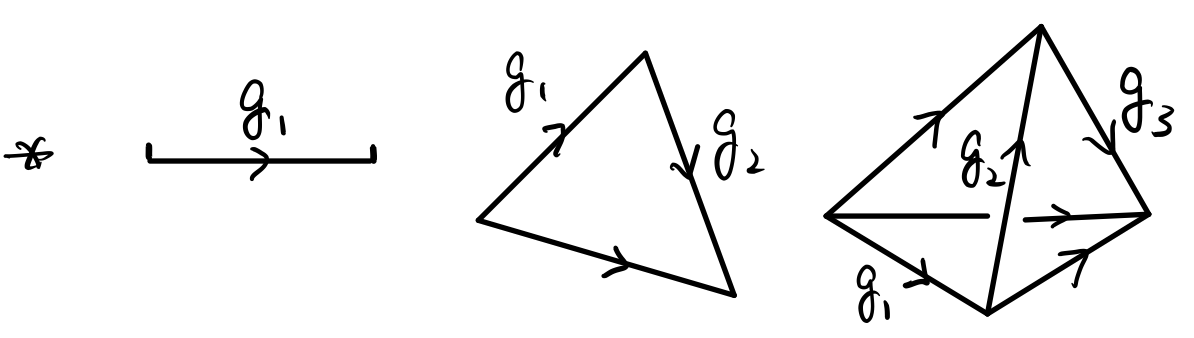
\includegraphics[height=2.5cm]{../chainmap/bg-std}}
    \visible<4->{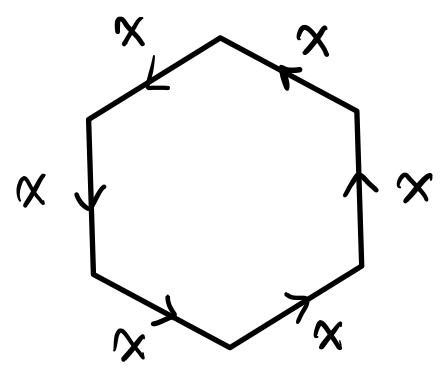
\includegraphics[height=2.5cm]{../chainmap/z6-1}}
  \end{center}
\end{frame}

\begin{frame}
  \frametitle{Examples of simplification}
 \begin{table}
    \centering
    %\renewcommand{\arraystretch}{1.5}
    \rowcolors{2}{black!20}{}
    \begin{tabularx}{\columnwidth}{xxxxxx}
      \rowcolor{mbg}\textcolor{white}{Group}
      &\textcolor{white}{$\dim C^1$}
      &\textcolor{white}{$\dim C^2$}
      &\textcolor{white}{$\dim C^3$}
      &\textcolor{white}{$\dim C^4$}
      &\textcolor{white}{$\dim C^5$}\\
      $\mathbb Z_n$ std & $n-1$ & $(n-1)^2$ & $(n-1)^3$ & $(n-1)^4$ & $(n-1)^5$\\
      $\mathbb Z_n$ red & 1 & 1 & 1 & 1 & 1\\
      $\mathbb D_n$ std & $2n-1$ & $(2n-1)^2$ & $(2n-1)^3$ & $(2n-1)^4$ & $(2n-1)^5$\\
      $\mathbb D_n$ red & 2 & 3 & 4 & 5 & 6\\
      p6mm std & $\infty$ & $\infty$ & $\infty$ & $\infty$ & $\infty$\\
      p6mm red & 5 & 13 & 25 & 41 & 60\\
    \end{tabularx}
  \end{table}  
\end{frame}

\begin{frame}
	\frametitle{Fermionic SPT: a generalized cohomology theory}
	\begin{itemize}
        \item An Atiyah–Hirzebruch Spectral Sequence: an fSPT state is specified by several layers.
          \[E^{pq}_2=H^p[G_b, \mathcal{H}_{\text{FSPT}}^q(\text{pt})]]\Rightarrow \mathcal{H}_{\text{FSPT}}^{p+q}(BG_b).\]
        \item Example: 2D fSPT,
          \begin{enumerate}
          \item $n_1\in H^1[G, \mathbb Z_2]$: Majorana-chain decoration.
          \item $n_2\in C^2[G, \mathbb Z_2]$: Complex-fermion decoration.
          \item $\nu_3\in C^3[G, \uone]$: Bosonic phase factor.
          \item A real-space construction: Q-R Wang and Z-C Gu, PRX 2020.
          \end{enumerate}
	\end{itemize}

        \begin{center}
          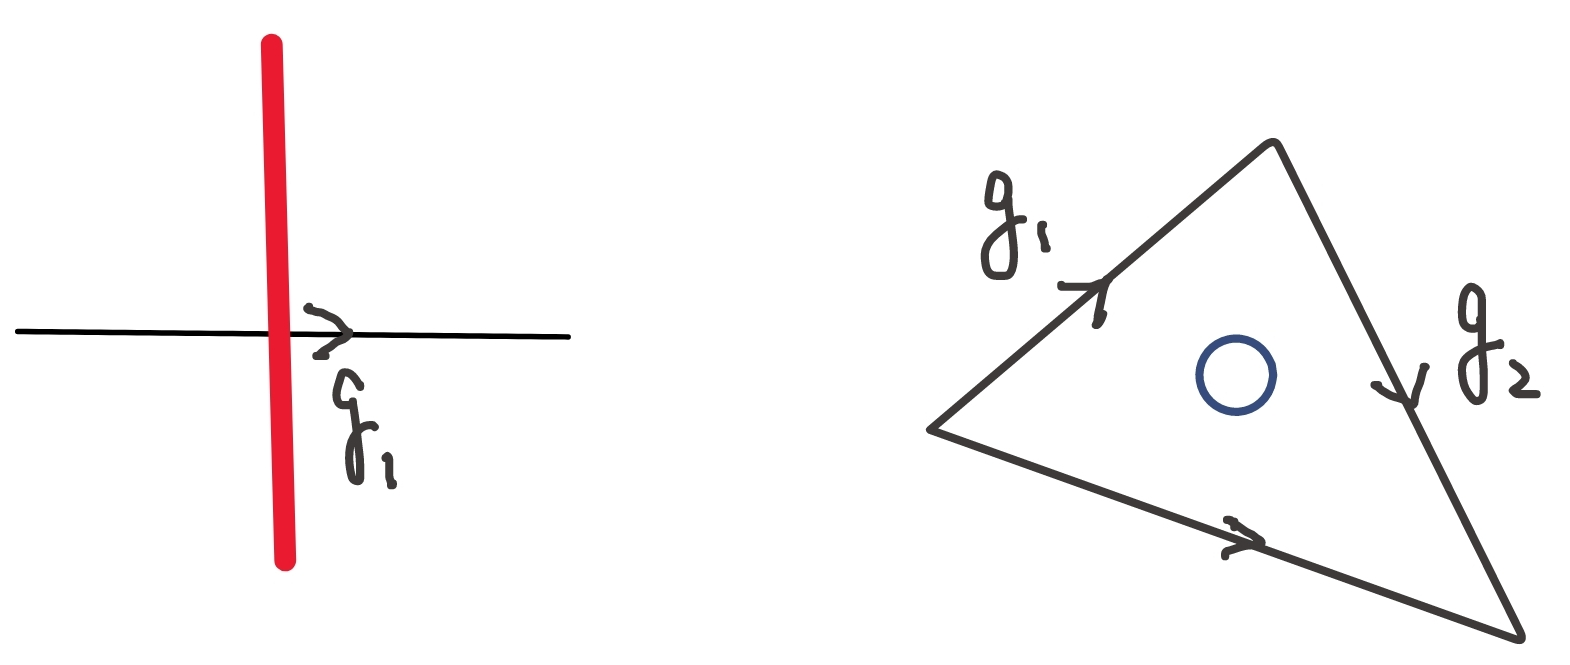
\includegraphics[height=3cm]{fspt_decor}
        \end{center}
\end{frame}

\begin{frame}
	\frametitle{Fermionic SPT: a generalized cohomology theory}
	\begin{itemize}
		\item Obstruction functions: higher-page derivatives of the spectral sequence.
		\item Example: checking if $n_1\in H^1[G, \mathbb Z_2]$ is obstructed?
		\begin{enumerate}
			\item Check $\mathcal O_3[n_1] = \omega_2\cup n_1 + s_1\cup n_1\cup n_1$ vanishes.
			\item Find $n_2$ such that $dn_2 = \mathcal O_3[n1]$.
			\item Check $\mathcal O_4[n_2]$ vanishes.
			\begin{align*}\mathcal O_4(01234) = \frac12\big[\omega_2\cup n_2 + n_2\cup n_2 + n_2 \cup_1 dn_2 + \omega_2(013)dn_2(1234)\\ + dn_2(0124)dn_2(0234)\big]
			-\frac14\big\{dn_2(0123)[1-dn_2(0124)]\text{ (mod 2)}\big\}.
		\end{align*}
		\end{enumerate}
		This defines a map between cohomology classes
		$C^1\rightarrow C^4:n_1\mapsto \mathcal O_4$.
		\item Acceleration: use basis transformation $\tilde C^1\rightarrow C^1\rightarrow C^4\rightarrow\tilde C^4$.
	\end{itemize}
\end{frame}

%\begin{frame}[fragile]
%	\frametitle{GAP, HAP and group cohomology}
%	\begin{itemize}
%		\item bSPT: $H^D[G,\uone]$ can be computed directly using HAP in GAP.
%		\item $H^D[G,\uone]$ ``='' $H^{D+1}[G,\mathbb Z]$. \emph{See X-G Wen, PRB \textbf{91}, 205101 (2015)}
%	\end{itemize}
%	\begin{columns}
%		\column{.5\columnwidth}
%	\begin{lstlisting}[basicstyle=\footnotesize]
%gap> LoadPackage("HAP");
%gap> G := CyclicGroup(4);
%pc group of size 4 with 2 generators>
%gap> GroupCohomology(G, 2);
%[ 4 ]
%gap> GroupCohomology(G, 3);
%[  ]
%gap> GroupCohomology(G, 4);
%[ 4 ]
%gap> GroupCohomology(G, 5);
%[  ]
%\end{lstlisting}
%	\column{.5\columnwidth}
%	\[H^{2n+1}[\mathbb Z_4,\uone] = \mathbb Z_4\]
%	\[H^{2n}[\mathbb Z_4,\uone] = \mathbb Z_1\]
%	\end{columns}
%\end{frame}

\begin{frame}[fragile]
	\frametitle{Implimenting chain maps in GAP}
	\begin{itemize}
		\item We are working on a GAP package to impliment the chain maps and to compute fSPT classifications.
		\item User only need to input the mappingin terms of inhomogeneous cocycles.
		\item The package automatically computes the mapping using the simplified resolution.
	\end{itemize}
\begin{lstlisting}[basicstyle=\footnotesize,morekeywords={function,return,local,if,fi,then,end},showspaces=false,showtabs=false, keywordstyle=\color{blue}]
SptSetInstallCoboundary(ss, 2, 2, 1,
function(n2, dn2)
  return function(g1, g2, g3, g4)
    local val;
    val := 1/2 * (n2(g1, g2) * n2(g3, g4) mod 2);
    if dn2 <> ZeroCocycle@ then
      val := val + 1/2 * ((n2(g1*g2*g3, g4) * dn2(g1, g2, g3)
        + n2(g1, g2*g3*g4) * dn2(g2, g3, g4)) mod 2);
      val := val + 1/2 * (dn2(g1, g2, g3*g4) * dn2(g1*g2, g3, g4) mod 2);
      val := val - 1/4 * (dn2(g1, g2, g3) * (1 - dn2(g1, g2, g3*g4)) mod 2);
    fi;
    return val;
  end;
end);
\end{lstlisting}
\end{frame}

%\begin{frame}[fragile]
%	\frametitle{Example: computing fSPT}
%	Consider 2D fSPT, $G=\mathbb Z_4$:
%\begin{lstlisting}[basicstyle=\footnotesize]
%gap> LoadPackage("SptSet");;
%gap> G := CyclicGroup(4);;
%gap> R := ResolutionFiniteGroup(G, 6);;
%gap> utAct := SptSetTrivialGroupAction(G);;
%gap> ss := FermionEZSPTSpecSeq(R, utAct);;
%gap> FermionSPTLayers(ss, 2);
%[ <ZL-Module with torsions [ 2 ]>, <ZL-Module with torsions [ 2 ]>,
%  <ZL-Module with torsions [ 4 ]> ]
%gap> z2tAct := GroupHomomorphismByImagesNC(G, GL(1, Integers),
%>   GeneratorsOfGroup(G), [ [[-1]], [[1]] ]);;
%gap> ss := FermionEZSPTSpecSeq(R, z2tAct);;
%gap> FermionSPTLayers(ss, 2);
%[ <ZL-Module with torsions [ 2 ]>, <ZL-Module []>, <ZL-Module []> ]
%\end{lstlisting}
%
%Example: compute fSPT for 2D wallpaper groups. (~10 min for all 17 groups.)
%\end{frame}
\begin{frame}
  \frametitle{Summary}
  \begin{itemize}
  %\item Use a simplified free resolution to accelerate computation of group cohomology.
  %\item Use chain maps between resolutions to compute maps between cohomology groups.
  \item We are working on a GAP package SptSet.
  \item Takes 5min to compute 2D fSPTs for all 17 wallpaper groups.
  \item Still missing some functions, which are unsolved in fSPT classification,
  \item Email me at \url{qiyang@fudan.edu.cn} for early access.
  %\item We also have a program written in python: faster but much harder to use.
  \item Will add more functions (fSPT with nontrivial group extension, group structure, ...), tweak the performence, and publish.
  \end{itemize}
\end{frame}

\section{Approach II: real-space construction}
% \section{Mathematical details}
\begin{frame}
	\frametitle{Decomposition of the space}
	We divide the space into finer cells such that
	\begin{enumerate}
		\item A cell $\sigma$ is maped to one single cell $\sigma^\prime$ under $SG$-action.
		\item $G_\sigma=\{g\in G|g:\sigma\rightarrow\sigma\}$ acts on $\sigma$ as onsite symmetry.
		\item A proper $G$-complex $Y\simeq \mathbb R^d$.
	\end{enumerate}
	\begin{columns}
		\column{.5\textwidth}
		\begin{center}
			\includegraphics[width=.5\textwidth]{../spspt/blocks}
		\end{center}
		\column{.5\textwidth}
		\begin{center}
			\begin{tikzpicture}
				\draw (-2, -2)--(-2, 2)--(2, 2)--(2, -2)--(-2, -2);
				\draw<2> [thick] (0, -2)--(0, 2);
				\draw [->] (.7, 0) arc (0:180:0.7);
				\filldraw (0, 0) circle (1pt) node [right] {$C_2$};
				\node<2> at (0, -1) [right] {$\tau_1$};
				\node<2> at (0, 1) [left] {$\tau_2$};
				\node<2> at (-1, 0) {$\sigma_1$};
				\node<2> at (1, 0) {$\sigma_2$};
			\end{tikzpicture}
		\end{center}
	\end{columns}
\end{frame}

\begin{frame}
	\frametitle{Topological crystalline states are made of building blocks}
	\begin{columns}
		\column{.4\textwidth}
		\begin{center}
			\includegraphics[width=\textwidth]{../spspt/blocks}
		\end{center}
		\column{.6\textwidth}
		\begin{itemize}
			\item We divide the space into cells compatible with the space-group symmetry.
			\item On a $p$-cell $\sigma$, the SPT state is protected only by $G_\sigma$.
			\[\hat\omega(\sigma)\in \Phi^p(G_\sigma) = H^{p+1}[G_\sigma,\uone_T].\]
			\item $G_\sigma$ acts as onsite symmetries.
			\item Decorate 3d SPT on 3-cells; 2d SPT on 2-cells; 1d SPT on 1-cells; 0d SPT on 0-cells;
			\item $p$-block states: $E^p_{p,\infty}$.
			\[\text{TCSs} = ``\bigoplus_p\text{''} E^p_{p,\infty}.\]
		\end{itemize}
	\end{columns}
\end{frame}

%\begin{frame}
%	\frametitle{Symmetric conditions}
%	\begin{columns}
%		\column{.3\textwidth}
%		\begin{tikzpicture}
%			\draw (0, 0)--(2, 0)--(2, 2)--(0, 2)--(0, 0);
%			\draw (2, 4)--(4, 4)--(4, 6)--(2, 6)--(2, 4);
%			\draw [thick,->] (1, 1) node [below] {$\hat\omega(\sigma$)} --
%			(3, 5) node [above] {$\hat\omega(\sigma^\prime)$};
%			\node at (2, 3) [right] {$g$};
%		\end{tikzpicture}
%		\column{.7\textwidth}
%		\begin{itemize}
%			\item If $g:\sigma\rightarrow\sigma^\prime$, then the cochains attached must be ``identical''.
%			\item $G_\sigma\neq G_{\sigma'}$, but they are isomorphic:
%			\[G_{\sigma'}=gG_\sigma g^{-1}\simeq G_\sigma.\]
%			\item This induces another isomorphism:
%			\[H^{p+1}[G_{\sigma'},\uone_T]\simeq H^{p+1}[G_\sigma,\uone_T]\]
%			\item $\hat\omega(\sigma)$ and $\hat\omega(\sigma')$ are related by this isomorphism
%			\[\hat\omega(\sigma') = g\cdot \hat\omega(\sigma).\]
%			\item Only decorations on symmetry-unrelated cells are independent: finite \# of them.
%		\end{itemize}
%	\end{columns}
%\end{frame}

\begin{frame}
	\frametitle{No-Open-Edge Conditions}
	\begin{columns}
		\column{.58\textwidth}
		\begin{itemize}
			\item<1-> SPT blocks have nontrivial boundary states.
			\item<2-> Boundary anomaly must cancel on $(p-1)$-cells.
			\item<3-> $\hat\omega(\sigma_1)
			+\hat\omega(\sigma_2)+\hat\omega(\sigma_3)+\hat\omega(\sigma_4)\simeq0$.
		\end{itemize}
		\column{.42\textwidth}
		\begin{tikzpicture}
			\draw (0, 1)--(-1, 1)--(-2, 0)--(2, 0)--(3, 1)--(1, 1);
			\draw [thick] (0, 0)--(1, 1);
			\draw<1-2> [string] (.2, .1)--(1, .9);
			\draw<1> [string] (1, .9)--(2.8, .9);
			\draw<1> [string] (2.8, .9)--(2, .1);
			\draw<1> [string] (2, .1)--(.2, .1);
			\draw<2> [string] (.1, .2)--(.9, 1);
			\draw<3-> [->] (1.3, .5)--(.6, .5);
			\draw<3-> [->] (.5, 1.3)--(.5, .6);
			\draw<3-> [->] (.5, -.3)--(.5, .4);
			\draw<3-> [->] (-.3, .5)--(.4, .5);
			\node<1-2> at (.5, .5) [above] {$\tau$};
			\node<3-> at (.7, .7) [above] {$\tau$};
			\draw (1, 1)--(1, 3)--(0, 2)--(0, -2)--(0, -2)--(1, -1)--(1, 0);
			\node at (.5, 1.5) {$\sigma_1$};
			\node at (1.5, .5) {$\sigma_2$};
			\node at (.5, -0.5) {$\sigma_3$};
			\node at (-0.5, .5) {$\sigma_4$};
		\end{tikzpicture}
	\end{columns}
\end{frame}

\begin{frame}
	\frametitle{Bubbling Equivalence}
\begin{columns}
\column{.7\textwidth}
\begin{itemize}
\item A bubbling process: fill a 2-cell with a loop of 1-dim SPT states.
\item Changes 1-cell decoration.
\item Does not change bulk classification.
\item Two decorations should be viewed as equivalent ones.
\end{itemize}
\column{.3\textwidth}
\begin{animateinline}{5}
        \multiframe{12}{Ra=.3+.05}{
\begin{tikzpicture}[scale=1]
	\draw (0, 0)--(2, 0)--(2, 2)--(0, 2)--(0, 0);
	\draw [dashed] (1, 2)--(1, 1)--(2, 1);
	\draw (2, 1)--(3, 1)--(3, 3)--(1, 3)--(1, 2);
	\draw [dashed] (0, 0)--(1, 1);
	\draw (2, 0)--(3, 1);
	\draw (0, 2)--(1, 3);
	\draw (2, 2)--(3, 3);
	\fill [blue!30,opacity=.5] (1.5-1.5*\Ra, 1.5-1.5*\Ra)--(1.5+0.5*\Ra, 1.5-1.5*\Ra)
	--(1.5+1.5*\Ra, 1.5-0.5*\Ra)--(1.5+1.5*\Ra, 1.5+1.5*\Ra)
	--(1.5-0.5*\Ra, 1.5+1.5*\Ra)--(1.5-1.5*\Ra, 1.5+0.5*\Ra)
	--(1.5-1.5*\Ra, 1.5-1.5*\Ra);
	\draw [blue,dashed] (1.5-1.5*\Ra, 1.5+0.5*\Ra)--(1.5+0.5*\Ra, 1.5+0.5*\Ra)--(1.5+1.5*\Ra,1.5+1.5*\Ra);
	\draw [blue,dashed] (1.5+0.5*\Ra, 1.5-1.5*\Ra)--(1.5+0.5*\Ra, 1.5+0.5*\Ra);
	\draw [->,thick] (1.5-0.5*\Ra, 1.5-0.5*\Ra)--(1.3-0.5*\Ra, 1.3-0.5*\Ra);
	\draw [->,thick] (1.5, 1.5+\Ra)--(1.5, 1.78+\Ra);
	\draw [->,thick] (1.5+\Ra, 1.5)--(1.78+\Ra, 1.5);
	%\fill [green!30] (-\Ra,-\Ra)--(-\Ra,\Ra)--(\Ra,\Ra)--(\Ra,-\Ra)--(-\Ra,-\Ra);
%\draw [blue,thick] (-\Ra,-\Ra)--(-\Ra,\Ra)--(\Ra,\Ra)--(\Ra,-\Ra)--(-\Ra,-\Ra);
%\node at (0, 0) {$d\nu$};
\end{tikzpicture}
}
\end{animateinline}
\end{columns}
\end{frame}

\begin{frame}
\frametitle{High-Order No-Open-Edge Conditions}
\begin{columns}
\column{.6\textwidth}
\begin{enumerate}
\item<1-> Choose a cocycle for each 2-cell $\sigma$.\\ Check $\partial\hat\omega_2(\tau)\simeq0$ for each 1-cell $\tau$.\\
\emph{1st-page no-open-edge condition.}
\item<2-> Choose a cochain $\hat\omega_1$ for each $\tau$.\\
Check $\partial\hat\omega_1(\lambda)\simeq0$ for each 0-cell $\lambda$.\\
\emph{2nd-page no-open-edge condition.}
\item<3> Choose a cochain $\hat\omega_0$ for each $\lambda$.
\end{enumerate}
\column{.4\textwidth}
\begin{center}
\begin{tikzpicture} [scale=3]
\fill [blue!50] (0,0)--(1,0)--(1.5,.5)--(1.5,1.5)--(0.5,1.5)--(0,1)--(0,0);
\draw<1> [thick,white] (0,0)--(1,0)--(1,1)--(0,1)--(0,0);
\draw<1> [thick,white] (1,0)--(1.5,.5)--(1.5,1.5)--(1,1);
\draw<1> [thick,white] (1.5,1.5)--(0.5,1.5)--(0,1);
\draw<1> [thick,white] (0,0)--(.5,.5)--(.5,1.5);
\draw<1> [thick,white](.5,.5)--(1.5,.5);
\draw<2-> [thick,red] (0,0)--(1,0)--(1,1)--(0,1)--(0,0);
\draw<2-> [thick,red] (1,0)--(1.5,.5)--(1.5,1.5)--(1,1);
\draw<2-> [thick,red] (1.5,1.5)--(0.5,1.5)--(0,1);
\draw<2-> [thick,red] (0,0)--(.5,.5)--(.5,1.5);
\draw<2-> [thick,red](.5,.5)--(1.5,.5);
\fill<1-2> [white] (0,0) circle (2pt);
\fill<1-2> [white] (1,0) circle (2pt);
\fill<1-2> [white] (0,1) circle (2pt);
\fill<1-2> [white] (1,1) circle (2pt);
\fill<1-2> [white] (0.5,0.5) circle (2pt);
\fill<1-2> [white] (1.5,0.5) circle (2pt);
\fill<1-2> [white] (0.5,1.5) circle (2pt);
\fill<1-2> [white] (1.5,1.5) circle (2pt);
\fill<3> [red] (0,0) circle (2pt);
\fill<3> [red] (1,0) circle (2pt);
\fill<3> [red] (0,1) circle (2pt);
\fill<3> [red] (1,1) circle (2pt);
\fill<3> [red] (0.5,0.5) circle (2pt);
\fill<3> [red] (1.5,0.5) circle (2pt);
\fill<3> [red] (0.5,1.5) circle (2pt);
\fill<3> [red] (1.5,1.5) circle (2pt);
\end{tikzpicture}
\end{center}
\end{columns}
Higher-page computations are organized as a spectral sequence.
\end{frame}

%\begin{frame}
%	\frametitle{A building block}
%	\begin{columns}
%		\column{.4\textwidth}
%		\begin{center}
%			\includegraphics[width=\textwidth]{blocks}
%		\end{center}
%		\column{.6\textwidth}
%		\begin{itemize}
%			\item A building block $\hat\omega$ is a collection of cochains:
%			\[\hat\omega(\sigma) \in C^{p+1}[G_\sigma, \uone_T].\]
%			\item $\hat\omega$ needs to be symmetric under $SG$.
%			\item $\hat\omega$ needs to satisfy the bulk-boundary relation:
%			\[d\hat\omega(\tau) = \sum_{\sigma:\tau\in\partial\sigma}\hat\omega(\sigma).\]
%			\item Need to find when two blocks can be deformed to each other: $\hat\omega\simeq\hat\omega^\prime$.
%		\end{itemize}
%	\end{columns}
%\end{frame}

\begin{frame}
\frametitle{Mathematical Proof for bosonic SPTs}
\begin{itemize}
\item Equivariant group cohomology:
\[H^{d+1}[G, \uone_{PT}]]\simeq H^{d+1}_G[X, \uone_{PT}].\]
Here $X\sim\text{pt}$ is a (non-free) $G$-complex. See Thorngren and Else, PRX (2018).
\item There is a spectral sequence:
\[E_1^{pq}=\bigoplus_{\sigma\in X_p/G}H^q[G_\sigma,\uone_T]\Rightarrow
 H^{p+q}[G, \uone_{PT}]].\]
See Kenneth S. Brown's book, Chapter VII.
\item The topological space $Y$ we used is the Poincar\'e dual of $X$: $E^{pq}_r\simeq E^{q-1}_{d-p,r}$
\end{itemize}
\begin{center}
	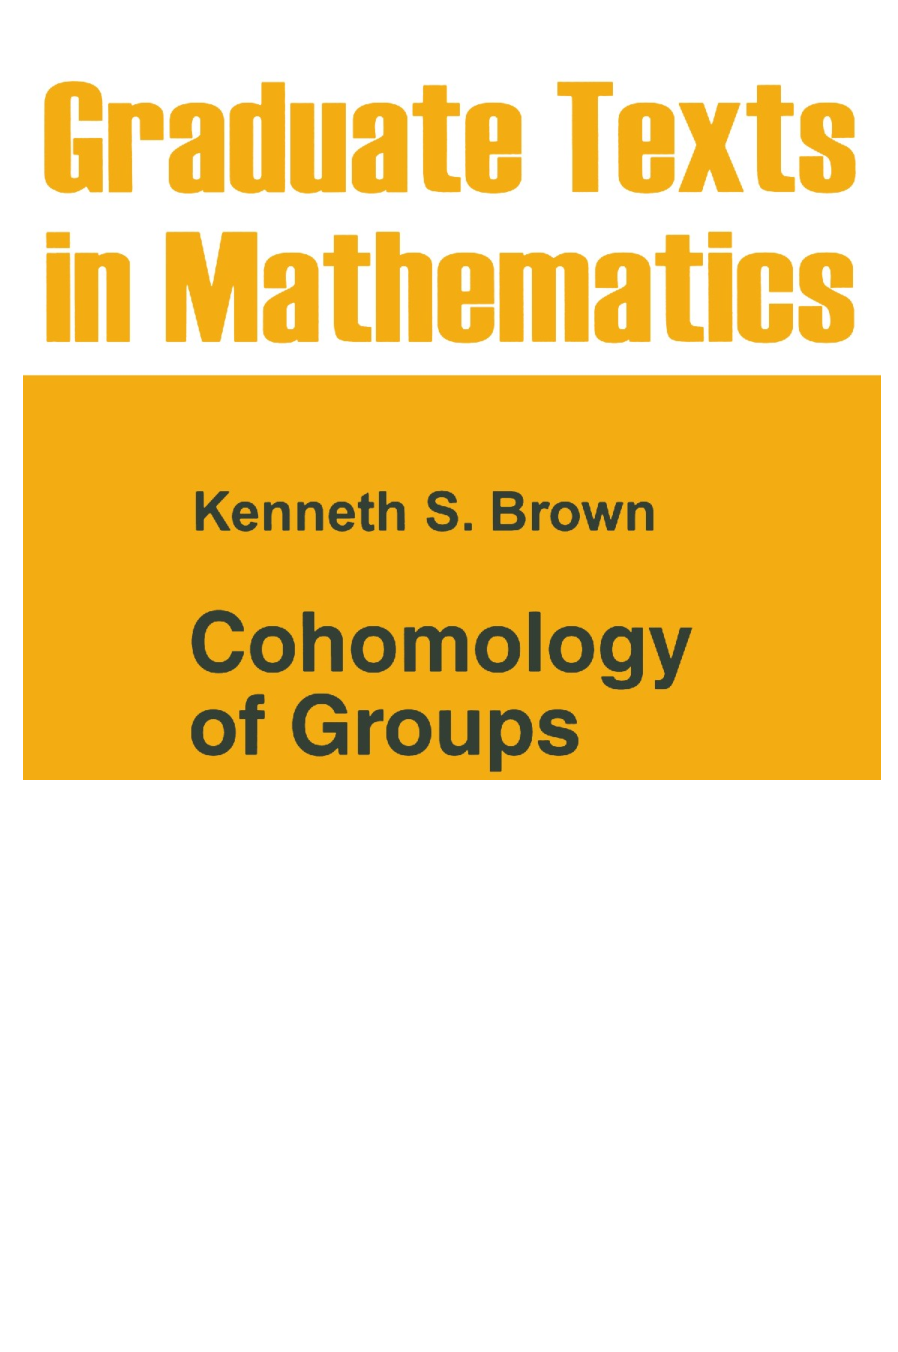
\includegraphics[height=2cm]{brown_book}
	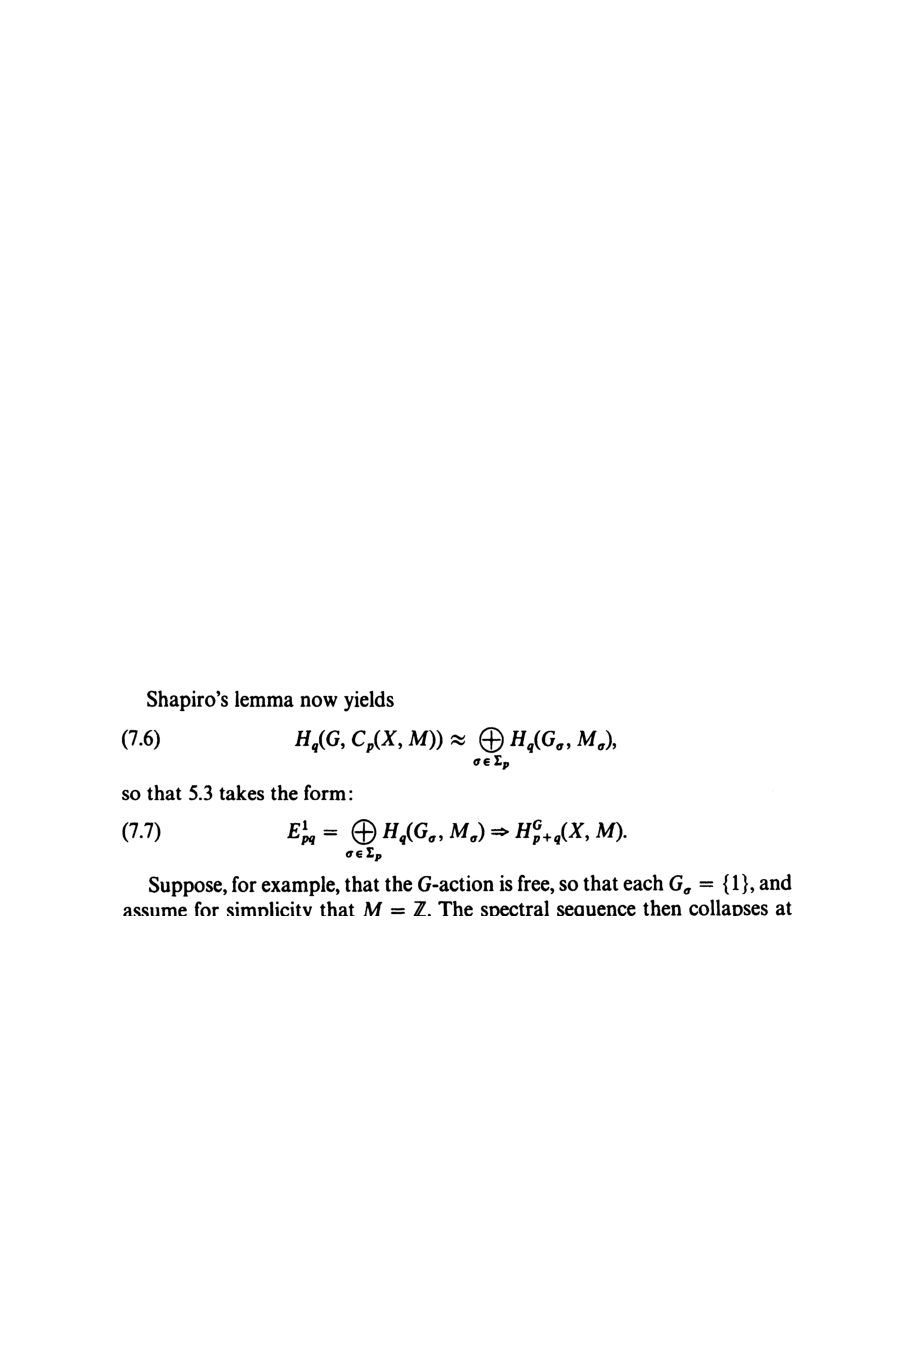
\includegraphics[height=2cm]{brown_ss}
\end{center}
\end{frame}

\begin{frame}
  \frametitle{Real-space construction of fSPTs}

  \begin{itemize}
  \item Jian-Hao Zhang, Shuo Yang, YQ and Zheng-Cheng Gu, arXiv:2012.15657
  \item Need to decorate complex fermions, Kitaev chains, etc.
  \item We computed fSPT classification protected by 17 wallpaper groups, and the two approaches agree.
  %\item Still need automated programs for real-space construction of fSPTs.
  \end{itemize}
  \begin{center}
    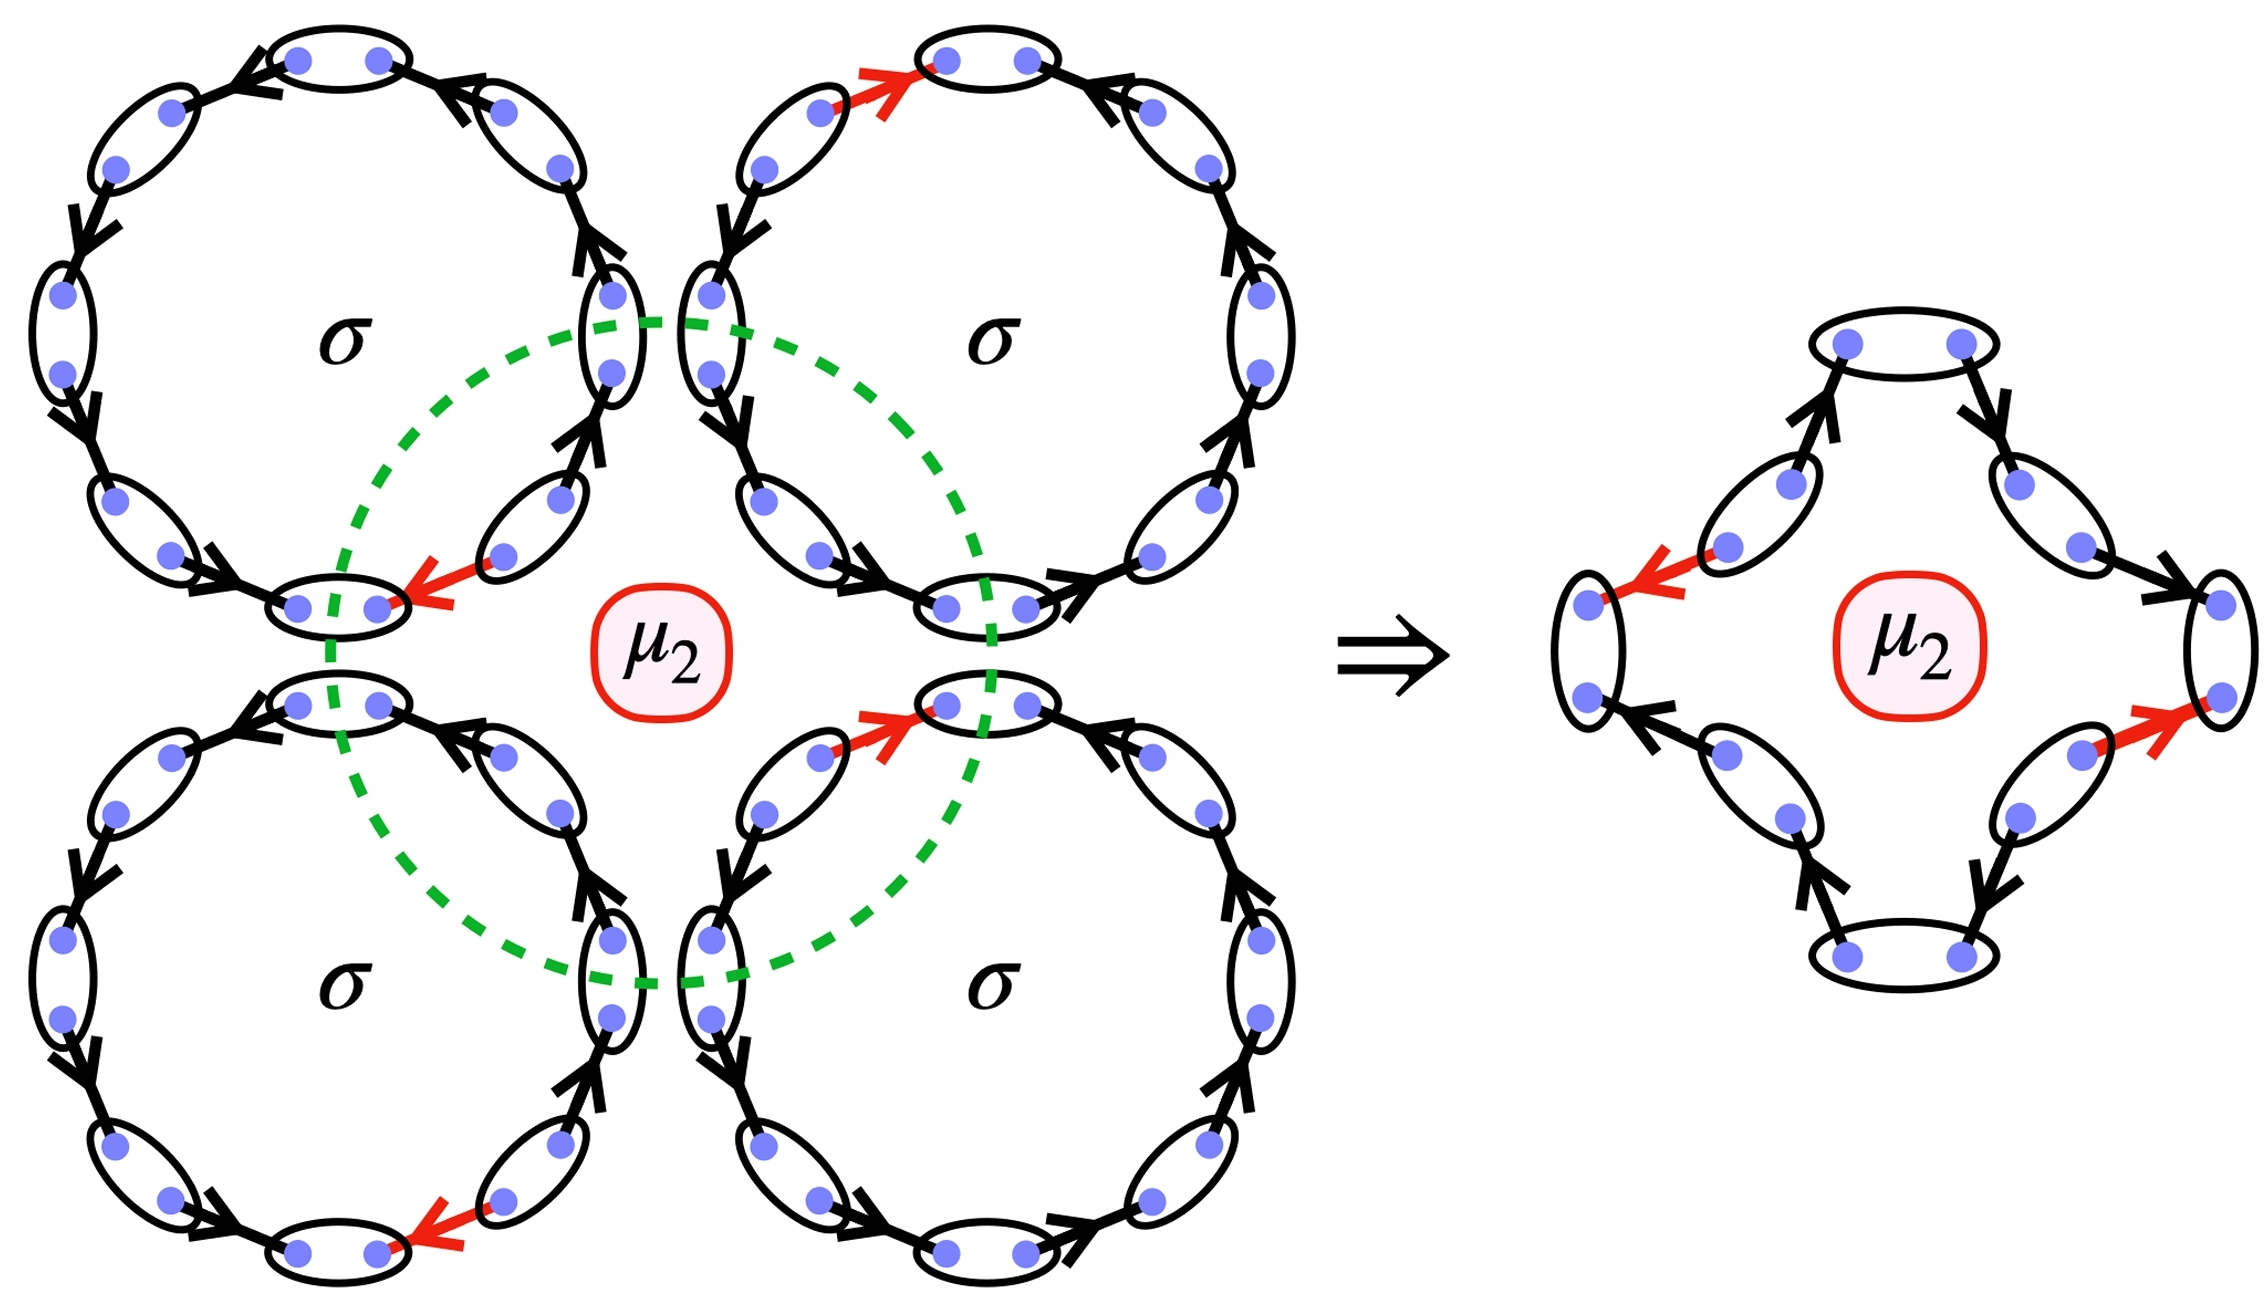
\includegraphics[height=4cm]{majorana_bubble}    
  \end{center}
\end{frame}

\section{Conclusion}

\begin{frame}
  \frametitle{Some related works}
  \begin{itemize}
  \item The chain maps to/from bar resolution is used to compute the homology groups of the classifying space of 2-groups.\\
    Graham Ellis and Le Van Luyen, J. Symb. Comput. \textbf{47}, 1309 (2012).
  \item fSPT of point-group symmetries:
    M Cheng and C Wang, arXiv:1810.12308.
  \item Another work about spectral sequence: Ken Shiozaki, Masatoshi Sato and Kiyonori Gomi, arXiv:1802.06694 (momentum-space analysis).
  \item An independent work: Else and Thorngren, arXiv:1810.10539.
  \item Related work: K. Shiozaki, C. Zhaoxi Xiong, and K. Gomi,
    arXiv:1810.00801.
  \end{itemize}
\end{frame}

\begin{frame}
\frametitle{Summary: towards a complete classification of fSPTs}
\begin{itemize}
\item Onsite symmetry: 1D \ding{51}, 2D \ding{51}, 3D ??.
\item Crystalline symmetry: treat as onsite symmetry / real-space construction.
  \begin{itemize}
  \item Some missing formulas in onsite-symmetry fSPT classification?
  \item General rules and automated programs of real-space construction for fSPTs?
  \end{itemize}
\end{itemize}
\end{frame}

\end{document}
